\documentclass[9pt,aspectratio=169]{beamer}

\usetheme[numbering=fraction,progressbar=foot]{metropolis}

\usepackage[T1]{fontenc}
\usepackage{lmodern}
\usepackage{microtype}
\usepackage{booktabs}
\usepackage{tabularx}
\usepackage{array}
\usepackage{graphicx}
\usepackage{tikz}
\usepackage{amsmath}
\usepackage{amssymb}
\usepackage{attachfile2}
\usepackage{multimedia}
\usepackage{openmoji}

\usetikzlibrary{arrows.meta,calc,positioning,shapes.geometric,fit,backgrounds}

\definecolor{Ink}{HTML}{1F2937}
\definecolor{Muted}{HTML}{6B7280}
\definecolor{Sand}{HTML}{F7F4EC}
\definecolor{Gold}{HTML}{C27D38}
\definecolor{Teal}{HTML}{147A73}
\definecolor{Sage}{HTML}{6B8F71}
\definecolor{Rose}{HTML}{C85C5C}
\definecolor{Paper}{HTML}{FFFDF8}
\definecolor{Mist}{HTML}{E8F1EF}
\definecolor{Peach}{HTML}{F6E4D8}
\definecolor{Slate}{HTML}{DDE4EC}
\definecolor{Night}{HTML}{0F172A}

\setbeamercolor{normal text}{fg=Ink,bg=Sand}
\setbeamercolor{frametitle}{fg=Ink,bg=Sand}
\setbeamercolor{progress bar}{fg=Gold,bg=Slate}
\setbeamercolor{title separator}{fg=Gold}
\setbeamercolor{alerted text}{fg=Gold}
\setbeamercolor{footnote}{fg=Muted}

\setbeamertemplate{navigation symbols}{}
\setbeamersize{text margin left=0.75cm,text margin right=0.75cm}

\title{Music Style Transfer and\\Deep Generative Genre Remastering}
\subtitle{A 50-minute technical lecture followed by a DGGR case study}
\author{Sahara Kaul \and Kelsey Pattison \and Ahmed Sajid}
\date{CMPUT 414, Winter 2026}

\newcommand{\cardbox}[2]{%
  \begin{tikzpicture}
    \node[
      fill=#1,
      rounded corners=14pt,
      inner xsep=11pt,
      inner ysep=9pt,
      text width=\dimexpr\linewidth-22pt\relax,
      align=left
    ] {\strut #2};
  \end{tikzpicture}%
}

\newcommand{\tagpill}[2]{%
  \tikz[baseline=(x.base)]\node[
    fill=#1,
    rounded corners=7pt,
    inner xsep=7pt,
    inner ysep=3.5pt
  ] (x) {\scriptsize\bfseries #2};%
}

\newcommand{\sectionbanner}[2]{%
  \begin{frame}[plain]
  \begin{tikzpicture}[remember picture,overlay]
    \fill[#1] (current page.south west) rectangle (current page.north east);
    \fill[white,opacity=0.12] ($(current page.north east)+(-1.2,-1.0)$) circle (2.4cm);
    \fill[white,opacity=0.10] ($(current page.south west)+(1.0,0.8)$) circle (1.8cm);
  \end{tikzpicture}
  \vfill
  {\color{white}\usebeamerfont{title}#2\par}
  \vspace{0.25cm}
  {\color{white!85}\Large Lecture section}
  \vfill
  \end{frame}
}

\newcommand{\AudioButton}[3]{%
  \movie[showcontrols]%
    {\fcolorbox{Gold}{Paper}{\strut\scriptsize Play}}%
    {#1}%
  \hspace{0.35em}%
  \attachfile[color=Teal]{#1}%
  \hspace{0.45em}%
  {\scriptsize #2 \textcolor{Muted}{(#3)}}%
}

\newcommand{\refstrip}[1]{{\tiny\color{Muted}#1}}

\begin{document}

\begin{frame}[plain]
\begin{tikzpicture}[remember picture,overlay]
  \fill[Teal!20] ($(current page.south west)+(-0.6,0.4)$) circle (2.8cm);
  \fill[Gold!25] ($(current page.north east)+(-0.8,-0.8)$) circle (2.5cm);
  \fill[Rose!12] ($(current page.north west)+(1.4,-0.7)$) circle (1.4cm);
\end{tikzpicture}

\vspace{0.35cm}
\begin{columns}[T,onlytextwidth]
  \column{0.61\textwidth}
  {\usebeamerfont{title}\color{Ink}\inserttitle\par}
  \vspace{0.24cm}
  {\large\color{Muted}\insertsubtitle\par}
  \vspace{0.45cm}
  {\normalsize\insertauthor\par}
  {\small\color{Muted}\insertdate\par}
  \vspace{0.45cm}
  {\small
    \tagpill{Mist}{Part I}
    \hspace{0.35em}
    general lecture: problem framing, theory, representations, models, and evaluation
  }
  \par\vspace{0.18cm}
  {\small
    \tagpill{Peach}{Part II}
    \hspace{0.35em}
    DGGR case study: what we built, what worked, what still fails, and embedded audio
  }

  \column{0.39\textwidth}
  \cardbox{Paper}{
    \textbf{\openmoji[height=1.5ex]{musical score} Goal}\\[-0.2em]
    \small
    Treat this as a lecture first. We will start from the field itself, then use our repo as a concrete implementation example near the end.
  }
  \vspace{0.2cm}
  \cardbox{Mist}{
    \textbf{\openmoji[height=1.5ex]{headphone} Media note}\\[-0.2em]
    \small
    Audio clips are embedded and also attached to the PDF. Acrobat-compatible viewers handle inline playback most reliably.
  }
\end{columns}
\end{frame}

\begin{frame}{Talk Structure}
\begin{columns}[T,onlytextwidth]
  \column{0.5\textwidth}
  \cardbox{Mist}{
    \textbf{Part I: general lecture}\\[-0.2em]
    \small
    Motivation, definitions, historical context, core model families, evaluation criteria, and the main failure modes in music style transfer.
  }
  \vspace{0.2cm}
  \cardbox{Peach}{
    \textbf{Part II: DGGR case study}\\[-0.2em]
    \small
    Architecture, lab-by-lab progress, saved-run evidence, audio demos, creative elements, and realistic next steps.
  }

  \column{0.5\textwidth}
  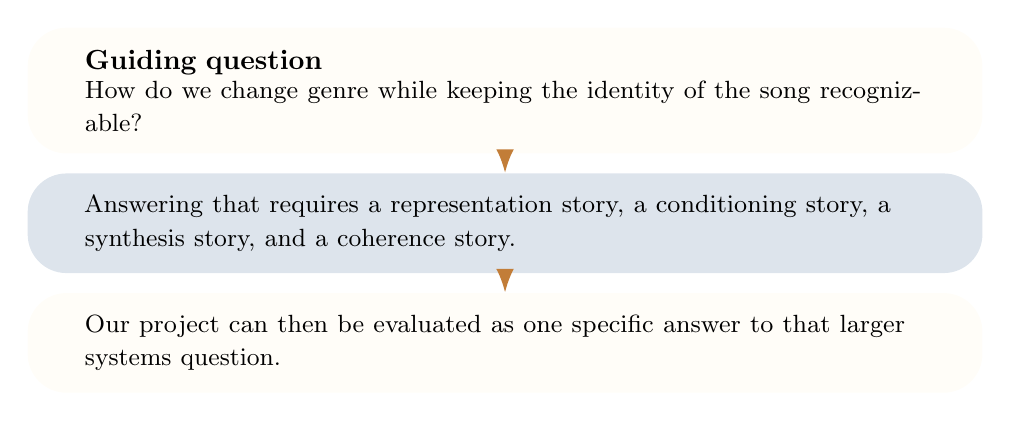
\begin{tikzpicture}[>=Latex, node distance=0.24cm]
    \node[fill=Paper, rounded corners=14pt, minimum width=\linewidth, text width=0.88\linewidth, inner xsep=12pt, inner ysep=8pt] (a) {
      \textbf{Guiding question}\\[-0.15em]
      \small
      How do we change genre while keeping the identity of the song recognizable?
    };
    \node[fill=Slate, rounded corners=14pt, minimum width=\linewidth, text width=0.88\linewidth, inner xsep=12pt, inner ysep=8pt, below=of a] (b) {
      \small
      Answering that requires a representation story, a conditioning story, a synthesis story, and a coherence story.
    };
    \node[fill=Paper, rounded corners=14pt, minimum width=\linewidth, text width=0.88\linewidth, inner xsep=12pt, inner ysep=8pt, below=of b] (c) {
      \small
      Our project can then be evaluated as one specific answer to that larger systems question.
    };
    \draw[-{Latex[length=3mm]}, thick, color=Gold] (a.south) -- (b.north);
    \draw[-{Latex[length=3mm]}, thick, color=Gold] (b.south) -- (c.north);
  \end{tikzpicture}
\end{columns}
\end{frame}

\sectionbanner{Night}{Part I\\General Lecture}

\begin{frame}{Motivation: Why This Problem Is Hard}
\begin{columns}[T,onlytextwidth]
  \column{0.5\textwidth}
  \cardbox{Peach}{
    \textbf{\openmoji[height=1.4ex]{speaker high volume} Audio is unforgiving}\\[-0.2em]
    \small
    Small errors in phase, transients, or continuity are immediately audible. Artifacts that might be tolerated in images are distracting in music.
  }
  \vspace{0.2cm}
  \cardbox{Mist}{
    \textbf{\openmoji[height=1.4ex]{brain} Music is multilevel}\\[-0.2em]
    \small
    Melody, rhythm, harmony, instrumentation, arrangement, and production are entangled in the same signal.
  }

  \column{0.5\textwidth}
  \cardbox{Paper}{
    \textbf{The central mistake in weak systems}\\[-0.2em]
    \small
    A shallow timbre swap often changes surface texture without changing the deeper musical organization. The result sounds processed, not re-conceived.
  }
  \vspace{0.2cm}
  \cardbox{Slate}{
    \textbf{What a stronger system must do}\\[-0.2em]
    \small
    1. Isolate content from style.\\
    2. Encode a target genre in a controllable form.\\
    3. Synthesize realistic audio.\\
    4. Preserve coherence over long horizons.
  }
\end{columns}

\vspace{0.08cm}
\refstrip{Lecture framing grounded in Dai et al. (2018), Hung et al. (2019), and Yang et al. (2019).}
\end{frame}

\begin{frame}{Problem Statement and Success Criteria}
\begin{columns}[T,onlytextwidth]
  \column{0.56\textwidth}
  \begin{equation*}
  x_{\text{src}} \;\longrightarrow\; \hat{x}_{\text{tgt}}
  \end{equation*}
  \begin{equation*}
  \begin{aligned}
  \text{subject to}\quad
  \mathrm{content}(\hat{x}_{\text{tgt}}) &\approx \mathrm{content}(x_{\text{src}}) \\
  \hat{x}_{\text{tgt}} &\in \mathcal{M}_{\text{genre=tgt}}
  \end{aligned}
  \end{equation*}
  \cardbox{Paper}{
    \textbf{Operational goal}\\[-0.2em]
    \small
    The output should sound as if the source had originally been arranged or performed in the target genre, not merely post-processed into it.
  }

  \column{0.44\textwidth}
  \cardbox{Mist}{
    \textbf{Three simultaneous objectives}\\[-0.2em]
    \small
    Content preservation\\
    Style/genre fidelity\\
    Acoustic realism
  }
  \vspace{0.2cm}
  \cardbox{Peach}{
    \textbf{Long-form adds a fourth}\\[-0.2em]
    \small
    Coherence across chunk boundaries, phrase structure, and minute-scale texture stability.
  }
\end{columns}
\end{frame}

\begin{frame}{Representation Levels in Music ML}
\begin{columns}[T,onlytextwidth]
  \column{0.58\textwidth}
  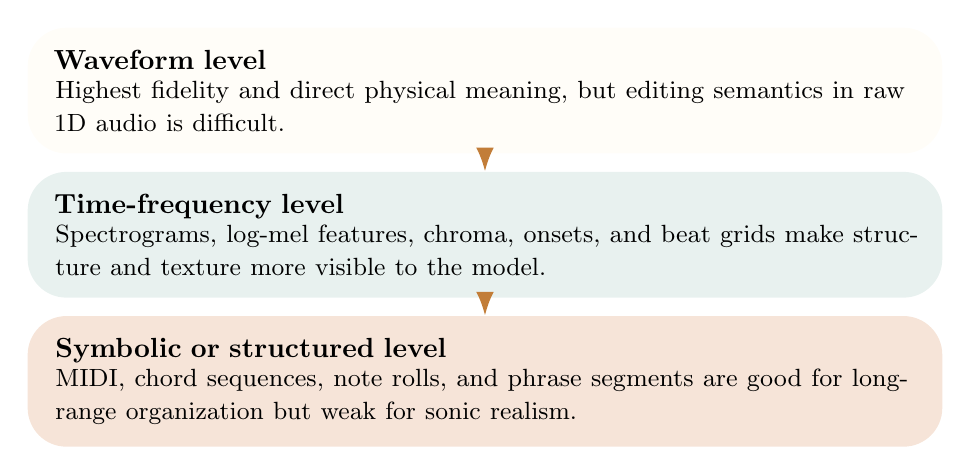
\begin{tikzpicture}[>=Latex, node distance=0.22cm]
    \node[fill=Paper, rounded corners=14pt, text width=0.9\linewidth, inner xsep=10pt, inner ysep=8pt] (a) {
      \textbf{Waveform level}\\[-0.15em]
      \small
      Highest fidelity and direct physical meaning, but editing semantics in raw 1D audio is difficult.
    };
    \node[fill=Mist, rounded corners=14pt, text width=0.9\linewidth, inner xsep=10pt, inner ysep=8pt, below=of a] (b) {
      \textbf{Time-frequency level}\\[-0.15em]
      \small
      Spectrograms, log-mel features, chroma, onsets, and beat grids make structure and texture more visible to the model.
    };
    \node[fill=Peach, rounded corners=14pt, text width=0.9\linewidth, inner xsep=10pt, inner ysep=8pt, below=of b] (c) {
      \textbf{Symbolic or structured level}\\[-0.15em]
      \small
      MIDI, chord sequences, note rolls, and phrase segments are good for long-range organization but weak for sonic realism.
    };
    \draw[-{Latex[length=3mm]}, thick, color=Gold] (a.south) -- (b.north);
    \draw[-{Latex[length=3mm]}, thick, color=Gold] (b.south) -- (c.north);
  \end{tikzpicture}

  \column{0.42\textwidth}
  \cardbox{Slate}{
    \textbf{Design lesson}\\[-0.2em]
    \small
    Strong systems usually combine levels. Structure is often easier to preserve in higher-level representations, while realism is recovered with a learned decoder, vocoder, or codec.
  }
  \vspace{0.2cm}
  \cardbox{Paper}{
    \textbf{Why this matters later}\\[-0.2em]
    \small
    Our repo follows this pattern directly: log-mel features for analysis, codec latents or mel diffusion for generation, and external decoders for waveform fidelity.
  }
\end{columns}
\end{frame}

\begin{frame}{What Do We Mean by Content, Style, and Genre?}
\begin{columns}[T,onlytextwidth]
  \column{0.33\textwidth}
  \cardbox{Peach}{
    \textbf{Content}\\[-0.2em]
    \small
    Melody, harmonic movement, rhythmic backbone, phrase placement, and whatever listeners still identify after instrumentation changes.
  }

  \column{0.33\textwidth}
  \cardbox{Mist}{
    \textbf{Style}\\[-0.2em]
    \small
    Timbre, articulation, groove feel, density, attack/decay behavior, production texture, and arrangement cues.
  }

  \column{0.34\textwidth}
  \cardbox{Paper}{
    \textbf{Genre}\\[-0.2em]
    \small
    A broader cultural and statistical manifold. No single acoustic feature defines it, but enough structure is learnable for classification and conditioning.
  }
\end{columns}

\vspace{0.2cm}
\begin{equation*}
x \mapsto \bigl(z_c, z_s\bigr),
\qquad
\text{genre} \approx \mathcal{G}(z_s,\text{context}),
\qquad
\hat{x} = D(z_c, z_{s,\mathrm{target}})
\end{equation*}
\end{frame}

\begin{frame}{Why Genre Is Especially Difficult}
\begin{columns}[T,onlytextwidth]
  \column{0.54\textwidth}
  \cardbox{Paper}{
    \textbf{Ill-defined but still learnable}\\[-0.2em]
    \small
    Genre depends on cultural convention, geography, era, production context, and listener expectation. That makes it semantically fuzzy, but not unusable in practice.
  }
  \vspace{0.2cm}
  \cardbox{Mist}{
    \textbf{What machine learning exploits}\\[-0.2em]
    \small
    Shared rhythmic, spectral, timbral, and arrangement statistics allow genre classifiers to work well even though genre itself is not reducible to one intrinsic feature.
  }

  \column{0.46\textwidth}
  \cardbox{Peach}{
    \textbf{Research consequence}\\[-0.2em]
    \small
    A generator should not treat genre as a one-hot texture label. It needs a richer target signal that captures a region of stylistic behavior.
  }
  \vspace{0.2cm}
  \cardbox{Slate}{
    \textbf{Evaluation consequence}\\[-0.2em]
    \small
    If the output is realistic but listeners would not place it in the target genre, the transfer still failed.
  }
\end{columns}

\vspace{0.08cm}
\refstrip{This slide follows Aucouturier and Pachet (2003) plus later genre-recognition work such as Ghosal and Kolekar (2018).}
\end{frame}

\begin{frame}{How We Evaluate a Style-Transfer System}
\small
\begin{tabularx}{\linewidth}{>{\raggedright\arraybackslash}p{3.0cm} >{\raggedright\arraybackslash}X >{\raggedright\arraybackslash}p{3.9cm}}
\toprule
\textbf{Axis} & \textbf{Question} & \textbf{Typical measurement} \\
\midrule
Content preservation & Does the melody / structural identity survive? & latent similarity, pitch correlation, MPS-style metrics \\
Style fidelity & Does the output move toward the target style? & classifier confidence, probe accuracy, centroid alignment \\
Audio realism & Does it sound plausible as audio? & adversarial critics, MR-STFT, FAD-like proxies, listening \\
Long-form coherence & Does it stay consistent over time? & boundary metrics, drift checks, human judgment \\
\bottomrule
\end{tabularx}

\vspace{0.18cm}
\cardbox{Paper}{
  \textbf{Important principle}\\[-0.2em]
  \small
  No single metric is sufficient. The best numeric checkpoint is often not the best listening checkpoint, especially in generative audio.
}
\end{frame}

\begin{frame}{Historical Evolution of the Field}
\small
\begin{tabularx}{\linewidth}{>{\raggedright\arraybackslash}p{2.8cm} >{\raggedright\arraybackslash}p{4.0cm} >{\raggedright\arraybackslash}X}
\toprule
\textbf{Era} & \textbf{Typical approach} & \textbf{Main weakness} \\
\midrule
Early transfer & Direct signal mapping, hand-crafted transforms, image-style analogies on spectrograms & Weak semantic control and strong artifact risk \\
Disentanglement wave & Separate pitch, rhythm, timbre, or content/style in latent space & Leakage is hard to eliminate and harder to verify \\
High-fidelity generation & GANs, neural codecs, universal vocoders, diffusion models & Better realism, but training and control are more complex \\
Long-form systems & Hierarchical latents, source anchoring, overlap constraints, chunk policies & Minute-scale drift and accumulation remain difficult \\
\bottomrule
\end{tabularx}

\vspace{0.18cm}
\begin{columns}[T,onlytextwidth]
  \column{0.5\textwidth}
  \cardbox{Mist}{
    \textbf{Trend}\\[-0.2em]
    \small
    The field moved away from single monolithic mappings toward staged systems with separate analysis, control, and synthesis modules.
  }
  \column{0.5\textwidth}
  \cardbox{Peach}{
    \textbf{Why that matters}\\[-0.2em]
    \small
    Once the problem is seen as multistage, engineering decisions become explicit rather than hidden inside one giant black box.
  }
\end{columns}
\end{frame}

\begin{frame}{Disentanglement as the First Core Tool}
\begin{columns}[T,onlytextwidth]
  \column{0.55\textwidth}
  \begin{equation*}
  E(x) \rightarrow \bigl(z_c, z_s\bigr)
  \end{equation*}
  \begin{equation*}
  \mathcal{L}_{\mathrm{content}} = \|z_c(x^{(a)}) - z_c(x^{(b)})\|_2^2
  \end{equation*}
  \begin{equation*}
  \mathcal{L}_{\mathrm{style}} = \mathrm{CE}(C_s(z_s), y_{\mathrm{style}})
  \end{equation*}
  \begin{equation*}
  \mathcal{L}_{\mathrm{adv}} = \mathrm{CE}(C_c(\mathrm{GRL}(z_c)), y_{\mathrm{style}})
  \end{equation*}

  \column{0.45\textwidth}
  \cardbox{Paper}{
    \textbf{Interpretation}\\[-0.2em]
    \small
    The content code is rewarded for staying stable across views and punished when style can be recovered from it. The style code is explicitly trained to remain style-bearing.
  }
  \vspace{0.2cm}
  \cardbox{Mist}{
    \textbf{Role of GRL}\\[-0.2em]
    \small
    The gradient reversal layer flips the adversarial signal so the encoder learns to hide style evidence from the content branch.
  }
\end{columns}
\end{frame}

\begin{frame}{Examples of Disentanglement Architectures}
\begin{columns}[T,onlytextwidth]
  \column{0.5\textwidth}
  \cardbox{Peach}{
    \textbf{DuoED / dual-encoder designs}\\[-0.2em]
    \small
    One encoder specializes in pitch or content, another in timbre or style, and multiple decoders force each latent to carry interpretable information.
  }
  \vspace{0.2cm}
  \cardbox{Mist}{
    \textbf{U-Net / skip-connection designs}\\[-0.2em]
    \small
    Let structural information bypass the bottleneck while style is learned in the latent path. This helps preserve pitch but can limit edit strength.
  }

  \column{0.5\textwidth}
  \cardbox{Paper}{
    \textbf{Sequence models and analogy systems}\\[-0.2em]
    \small
    GRU or VAE-based systems split latent dimensions into rhythm and pitch blocks so one can be changed while the other remains fixed.
  }
  \vspace{0.2cm}
  \cardbox{Slate}{
    \textbf{Practical lesson}\\[-0.2em]
    \small
    Architecture alone does not guarantee separation. You still need audits for style leakage, collapse, and downstream usefulness.
  }
\end{columns}
\end{frame}

\begin{frame}{Target Style Spaces and Genre Blueprints}
\begin{columns}[T,onlytextwidth]
  \column{0.55\textwidth}
  \begin{equation*}
  v_{\mathrm{target}} = \mathrm{normalize}\bigl([\alpha z_s \,\|\, \beta d]\bigr)
  \end{equation*}
  \begin{equation*}
  \mu_g = \frac{1}{|S_g|}\sum_{x \in S_g} v(x)
  \end{equation*}
  \cardbox{Paper}{
    \textbf{Idea}\\[-0.2em]
    \small
    The target genre is not a single example. It is a region or centroid in a style space built from many examples and optionally mixed with robust descriptors.
  }

  \column{0.45\textwidth}
  \cardbox{Mist}{
    \textbf{What makes a style space useful}\\[-0.2em]
    \small
    Linear separability, stable centroids, good nearest-neighbor behavior, and resistance to outliers or dataset imbalance.
  }
  \vspace{0.2cm}
  \cardbox{Peach}{
    \textbf{Failure mode}\\[-0.2em]
    \small
    If the style space is weak, the generator either ignores it or learns only a shallow edit.
  }
\end{columns}
\end{frame}

\begin{frame}{Conditioning Mechanisms: How the Target Signal Enters the Model}
\begin{columns}[T,onlytextwidth]
  \column{0.56\textwidth}
  \begin{equation*}
  \mathrm{FiLM}(F;c) = \gamma(c) \odot F + \beta(c)
  \end{equation*}
  \begin{equation*}
  \mathrm{AdaIN}(F;s) = \bigl(1+\gamma(s)\bigr) \odot \mathrm{IN}(F) + \beta(s)
  \end{equation*}
  \cardbox{Paper}{
    \textbf{Concept}\\[-0.2em]
    \small
    Rather than append the condition only at the input, modulation layers influence intermediate features throughout the network.
  }

  \column{0.44\textwidth}
  \cardbox{Mist}{
    \textbf{When FiLM is attractive}\\[-0.2em]
    \small
    Use it when a condition should steer a feature hierarchy across many depths and timescales.
  }
  \vspace{0.2cm}
  \cardbox{Peach}{
    \textbf{When separate style modulation helps}\\[-0.2em]
    \small
    If melody/structure and timbre/texture should not compete for the same path, FiLM and AdaIN can be separated by role.
  }
\end{columns}
\end{frame}

\begin{frame}{Generator Families: Strengths and Tradeoffs}
\small
\begin{tabularx}{\linewidth}{>{\raggedright\arraybackslash}p{2.5cm} >{\raggedright\arraybackslash}p{3.3cm} >{\raggedright\arraybackslash}X}
\toprule
\textbf{Family} & \textbf{Strength} & \textbf{Main tradeoff} \\
\midrule
Waveform GANs & Fast parallel generation and strong local realism when stable & Phase and local coherence are difficult; training can be brittle \\
Spectral GANs & Better phase handling in structured frequency domains & Need a reliable inversion / vocoding path \\
Neural codec editors & Decoder acts as a realism prior; easier than raw waveform synthesis & The latent space can constrain edit magnitude if the translator is too conservative \\
Diffusion models & Stable optimization and rich controllability & Slower inference; long-form consistency is still hard \\
\bottomrule
\end{tabularx}

\vspace{0.18cm}
\cardbox{Paper}{
  \textbf{Field-level takeaway}\\[-0.2em]
  \small
  There is no universally best generator. The choice depends on what matters more in the application: edit strength, fidelity, speed, or stability.
}
\end{frame}

\begin{frame}{Diffusion Models and Guided Editing}
\begin{columns}[T,onlytextwidth]
  \column{0.58\textwidth}
  \begin{equation*}
  q(x_t \mid x_0) = \mathcal{N}\!\left(\sqrt{\bar{\alpha}_t}\,x_0,\; (1-\bar{\alpha}_t)I\right)
  \end{equation*}
  \begin{equation*}
  v_t = \sqrt{\bar{\alpha}_t}\,\epsilon - \sqrt{1-\bar{\alpha}_t}\,x_0
  \end{equation*}
  \begin{equation*}
  \hat{\epsilon}_{\mathrm{cfg}}
  =
  \epsilon_\theta(x_t,t,\varnothing)
  + w\Bigl[\epsilon_\theta(x_t,t,c)-\epsilon_\theta(x_t,t,\varnothing)\Bigr]
  \end{equation*}

  \column{0.42\textwidth}
  \cardbox{Mist}{
    \textbf{Meaning of the equations}\\[-0.2em]
    \small
    The forward process adds noise, the reverse model learns to remove it, and classifier-free guidance controls how hard the condition pulls the sample toward the target.
  }
  \vspace{0.2cm}
  \cardbox{Peach}{
    \textbf{Why this is attractive for style transfer}\\[-0.2em]
    \small
    Guidance gives a direct knob over edit strength, which is especially useful when content preservation and genre shift compete.
  }
\end{columns}
\end{frame}

\begin{frame}{Long-Form Coherence: Why Generation Gets Harder Over Time}
\begin{columns}[T,onlytextwidth]
  \column{0.55\textwidth}
  \begin{equation*}
  x_t = \alpha(t)x_0 + \sigma(t)z, \qquad z \sim \mathcal{N}(0,I)
  \end{equation*}
  \cardbox{Paper}{
    \textbf{SDEdit intuition}\\[-0.2em]
    \small
    Start from a noised version of the source rather than from pure noise. This preserves macro-structure while still allowing local restyling.
  }
  \vspace{0.2cm}
  \cardbox{Mist}{
    \textbf{Chunking intuition}\\[-0.2em]
    \small
    Long songs are often generated in overlapping windows. The hard part is keeping those windows semantically aligned rather than merely crossfaded.
  }

  \column{0.45\textwidth}
  \cardbox{Peach}{
    \textbf{Failure modes}\\[-0.2em]
    \small
    Boundary seams, phrase drift, timbral inconsistency, warble accumulation, and eventual departure from the source melody.
  }
  \vspace{0.2cm}
  \cardbox{Slate}{
    \textbf{Useful controls}\\[-0.2em]
    \small
    Overlap locking, re-anchoring, source blending, hierarchical structure priors, and post-hoc seam diagnostics.
  }
\end{columns}
\end{frame}

\begin{frame}{General Design Rules Before We Look at Our Project}
\begin{columns}[T,onlytextwidth]
  \column{0.5\textwidth}
  \cardbox{Mist}{
    \textbf{Rule 1}\\[-0.2em]
    \small
    Do not ask one network to discover content, style, and waveform realism from scratch unless the data and compute budget justify it.
  }
  \vspace{0.2cm}
  \cardbox{Paper}{
    \textbf{Rule 2}\\[-0.2em]
    \small
    Measure each stage separately. A weak style space can make a strong generator look bad, and vice versa.
  }

  \column{0.5\textwidth}
  \cardbox{Peach}{
    \textbf{Rule 3}\\[-0.2em]
    \small
    Listening must be in the loop. For music generation, the best scalar metric is often not the best sounding checkpoint.
  }
  \vspace{0.2cm}
  \cardbox{Slate}{
    \textbf{Rule 4}\\[-0.2em]
    \small
    Long-form success is a systems problem involving generation policy, overlap handling, stabilization, and evaluation, not just one model choice.
  }
\end{columns}
\end{frame}

\sectionbanner{Teal}{Part II\\DGGR Case Study}

\begin{frame}{DGGR: Project Goal and Current Status}
\begin{columns}[T,onlytextwidth]
  \column{0.55\textwidth}
  \cardbox{Paper}{
    \textbf{Project thesis}\\[-0.2em]
    \small
    Deep Generative Genre Remastering treats genre transfer as a staged remastering problem: deconstruct the source, define a target blueprint, reconstruct realistic audio, then extend that to long-form coherence.
  }
  \vspace{0.2cm}
  \cardbox{Mist}{
    \textbf{Current repo-backed status}\\[-0.2em]
    \small
    Labs 1 through 4 are implemented and have saved artifacts. Lab 5 is the planned human evaluation layer and baseline comparison study.
  }

  \column{0.45\textwidth}
  \cardbox{Peach}{
    \textbf{How this maps to the lecture}\\[-0.2em]
    \small
    Lab 1 = disentanglement\\
    Lab 2 = target style space\\
    Lab 3 = reconstruction\\
    Lab 4 = long-form coherence\\
    Lab 5 = human validation
  }
  \vspace{0.2cm}
  \cardbox{Slate}{
    \textbf{What we will show}\\[-0.2em]
    \small
    Concrete architectures, metrics from the repo, and audio clips generated from saved runs.
  }
\end{columns}
\end{frame}

\begin{frame}{Full DGGR Pipeline}
\begin{columns}[T,onlytextwidth]
  \column{0.66\textwidth}
  \resizebox{\linewidth}{!}{%
  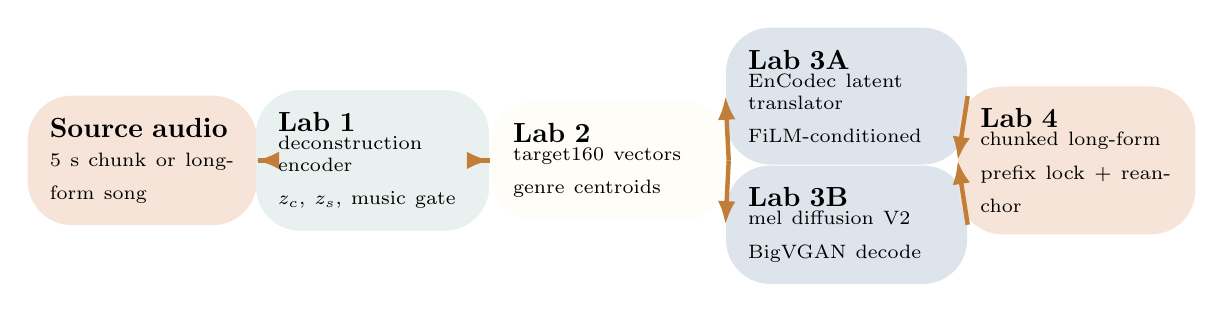
\begin{tikzpicture}[>=Latex, x=0.86cm, y=0.86cm]
    \node[fill=Peach, rounded corners=16pt, text width=2.35cm, inner xsep=8pt, inner ysep=8pt, align=left] (src) at (0,0) {
      \textbf{Source audio}\\[-0.15em]\scriptsize 5 s chunk or long-form song
    };
    \node[fill=Mist, rounded corners=16pt, text width=2.4cm, inner xsep=8pt, inner ysep=8pt, align=left] (lab1) at (3.4,0) {
      \textbf{Lab 1}\\[-0.15em]\scriptsize deconstruction encoder\\$z_c$, $z_s$, music gate
    };
    \node[fill=Paper, rounded corners=16pt, text width=2.45cm, inner xsep=8pt, inner ysep=8pt, align=left] (lab2) at (6.9,0) {
      \textbf{Lab 2}\\[-0.15em]\scriptsize target160 vectors\\genre centroids
    };
    \node[fill=Slate, rounded corners=16pt, text width=2.5cm, inner xsep=8pt, inner ysep=8pt, align=left] (codec) at (10.4,0.95) {
      \textbf{Lab 3A}\\[-0.15em]\scriptsize EnCodec latent translator\\FiLM-conditioned
    };
    \node[fill=Slate, rounded corners=16pt, text width=2.5cm, inner xsep=8pt, inner ysep=8pt, align=left] (diff) at (10.4,-0.95) {
      \textbf{Lab 3B}\\[-0.15em]\scriptsize mel diffusion V2\\BigVGAN decode
    };
    \node[fill=Peach, rounded corners=16pt, text width=2.45cm, inner xsep=8pt, inner ysep=8pt, align=left] (long) at (13.8,0) {
      \textbf{Lab 4}\\[-0.15em]\scriptsize chunked long-form\\prefix lock + reanchor
    };
    \draw[-{Latex[length=3mm]}, ultra thick, color=Gold] (src.east) -- (lab1.west);
    \draw[-{Latex[length=3mm]}, ultra thick, color=Gold] (lab1.east) -- (lab2.west);
    \draw[-{Latex[length=3mm]}, ultra thick, color=Gold] (lab2.east) -- (codec.west);
    \draw[-{Latex[length=3mm]}, ultra thick, color=Gold] (lab2.east) -- (diff.west);
    \draw[-{Latex[length=3mm]}, ultra thick, color=Gold] (codec.east) -- (long.west);
    \draw[-{Latex[length=3mm]}, ultra thick, color=Gold] (diff.east) -- (long.west);
  \end{tikzpicture}
  }

  \column{0.34\textwidth}
  \cardbox{Paper}{
    \textbf{Why staged?}\\[-0.2em]
    \small
    Each lab solves one of the general lecture problems explicitly instead of hoping one model learns all of them implicitly.
  }
  \vspace{0.2cm}
  \cardbox{Mist}{
    \textbf{Best current branch}\\[-0.2em]
    \small
    The codec translator is currently the strongest short-form result path. The diffusion branch is more ambitious and drives the long-form experiments.
  }
\end{columns}
\end{frame}

\begin{frame}{Data Universe and Label Risks}
\begin{columns}[T,onlytextwidth]
  \column{0.55\textwidth}
  \cardbox{Peach}{
    \textbf{What appears in the current workflow}\\[-0.2em]
    \small
    Baroque/classical renders, hip-hop material, lo-fi material, open-domain CC0 music, and speech negatives for the music gate.
  }
  \vspace{0.2cm}
  \cardbox{Paper}{
    \textbf{Observed genre buckets in the current Lab 2 run}\\[-0.2em]
    \small
    \texttt{baroque\_classical}: 411\\
    \texttt{cc0\_other}: 1200\\
    \texttt{hiphop\_xtc}: 1200\\
    \texttt{lofi\_hh\_lfbb}: 1200
  }

  \column{0.45\textwidth}
  \cardbox{Mist}{
    \textbf{Critical caveat}\\[-0.2em]
    \small
    Genre labels can accidentally encode dataset source. A model might learn recording or collection fingerprints instead of generalizable musical style.
  }
  \vspace{0.2cm}
  \cardbox{Slate}{
    \textbf{Why we say this explicitly}\\[-0.2em]
    \small
    Strong engineering presentations should surface confounds, not hide them. The repo docs already identify this as a real risk.
  }
\end{columns}
\end{frame}

\begin{frame}{Lab 1: Deconstruction Encoder Architecture}
\begin{columns}[T,onlytextwidth]
  \column{0.58\textwidth}
  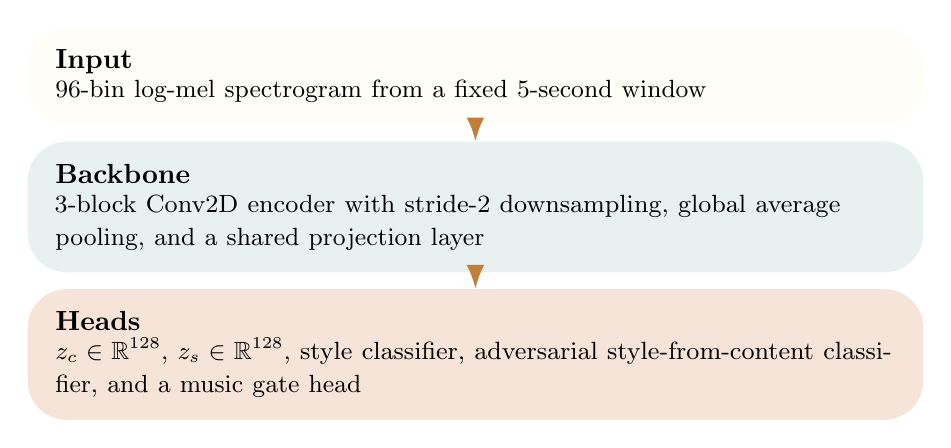
\begin{tikzpicture}[>=Latex, node distance=0.2cm]
    \node[fill=Paper, rounded corners=14pt, text width=0.88\linewidth, inner xsep=10pt, inner ysep=8pt] (a) {
      \textbf{Input}\\[-0.15em]
      \small 96-bin log-mel spectrogram from a fixed 5-second window
    };
    \node[fill=Mist, rounded corners=14pt, text width=0.88\linewidth, inner xsep=10pt, inner ysep=8pt, below=of a] (b) {
      \textbf{Backbone}\\[-0.15em]
      \small 3-block Conv2D encoder with stride-2 downsampling, global average pooling, and a shared projection layer
    };
    \node[fill=Peach, rounded corners=14pt, text width=0.88\linewidth, inner xsep=10pt, inner ysep=8pt, below=of b] (c) {
      \textbf{Heads}\\[-0.15em]
      \small $z_c \in \mathbb{R}^{128}$, $z_s \in \mathbb{R}^{128}$, style classifier, adversarial style-from-content classifier, and a music gate head
    };
    \draw[-{Latex[length=3mm]}, thick, color=Gold] (a.south) -- (b.north);
    \draw[-{Latex[length=3mm]}, thick, color=Gold] (b.south) -- (c.north);
  \end{tikzpicture}

  \column{0.42\textwidth}
  \cardbox{Slate}{
    \textbf{Training curriculum}\\[-0.2em]
    \small
    Phase 1 emphasizes content separation. Phase 2 increases adversarial pressure. Phase 3 sharpens the music gate and optionally uses a teacher anchor.
  }
  \vspace{0.2cm}
  \cardbox{Paper}{
    \textbf{Why this lab matters}\\[-0.2em]
    \small
    Every later module depends on the assumption that content and style have been separated well enough to recombine cleanly.
  }
\end{columns}
\end{frame}

\begin{frame}{Lab 1: Objective, Thresholds, and Outcome}
\begin{columns}[T,onlytextwidth]
  \column{0.58\textwidth}
  \begin{equation*}
  \mathcal{L}_{\mathrm{Lab1}}
  =
  \lambda_c \mathcal{L}_{\mathrm{content}}
  + \lambda_s \mathcal{L}_{\mathrm{style}}
  + \lambda_a \mathcal{L}_{\mathrm{adv}}
  + \lambda_g \mathcal{L}_{\mathrm{gate}}
  + \lambda_t \mathcal{L}_{\mathrm{anchor}}
  \end{equation*}
  \cardbox{Paper}{
    \textbf{Project thresholds}\\[-0.2em]
    \small
    style accuracy $\ge 0.85$\\
    content leakage $\le 0.15$\\
    gate ROC AUC $\ge 0.90$
  }

  \column{0.42\textwidth}
  \cardbox{Mist}{
    \textbf{Best observed audit}\\[-0.2em]
    \small
    style probe accuracy: \textbf{0.9417}\\
    content leakage above baseline: \textbf{0.1083}\\
    gate ROC AUC: \textbf{0.9299}
  }
  \vspace{0.2cm}
  \cardbox{Peach}{
    \textbf{Interpretation}\\[-0.2em]
    \small
    The lab clears its scientific gates. The remaining caution is calibration: an aggressive music-gate threshold can still trade recall for precision.
  }
\end{columns}
\end{frame}

\begin{frame}{Lab 2: Building the Target160 Space}
\begin{columns}[T,onlytextwidth]
  \column{0.46\textwidth}
  \begin{equation*}
  \mathrm{target160}
  =
  \mathrm{normalize}\bigl([2.0 \cdot z_s \,\|\, 1.0 \cdot d_{32}]\bigr)
  \end{equation*}
  \begin{equation*}
  d_{32} = [\mu_{1:16}, \sigma_{1:16}]
  \end{equation*}
  \cardbox{Paper}{
    \textbf{Construction logic}\\[-0.2em]
    \small
    The vector combines learned style information with simple mel-descriptor statistics, then builds per-genre centroids after inlier filtering.
  }
  \vspace{0.2cm}
  \cardbox{Mist}{
    \textbf{Why not just use a class label?}\\[-0.2em]
    \small
    A continuous target vector carries more structure than a one-hot tag and can support stronger conditional generation.
  }

  \column{0.54\textwidth}
  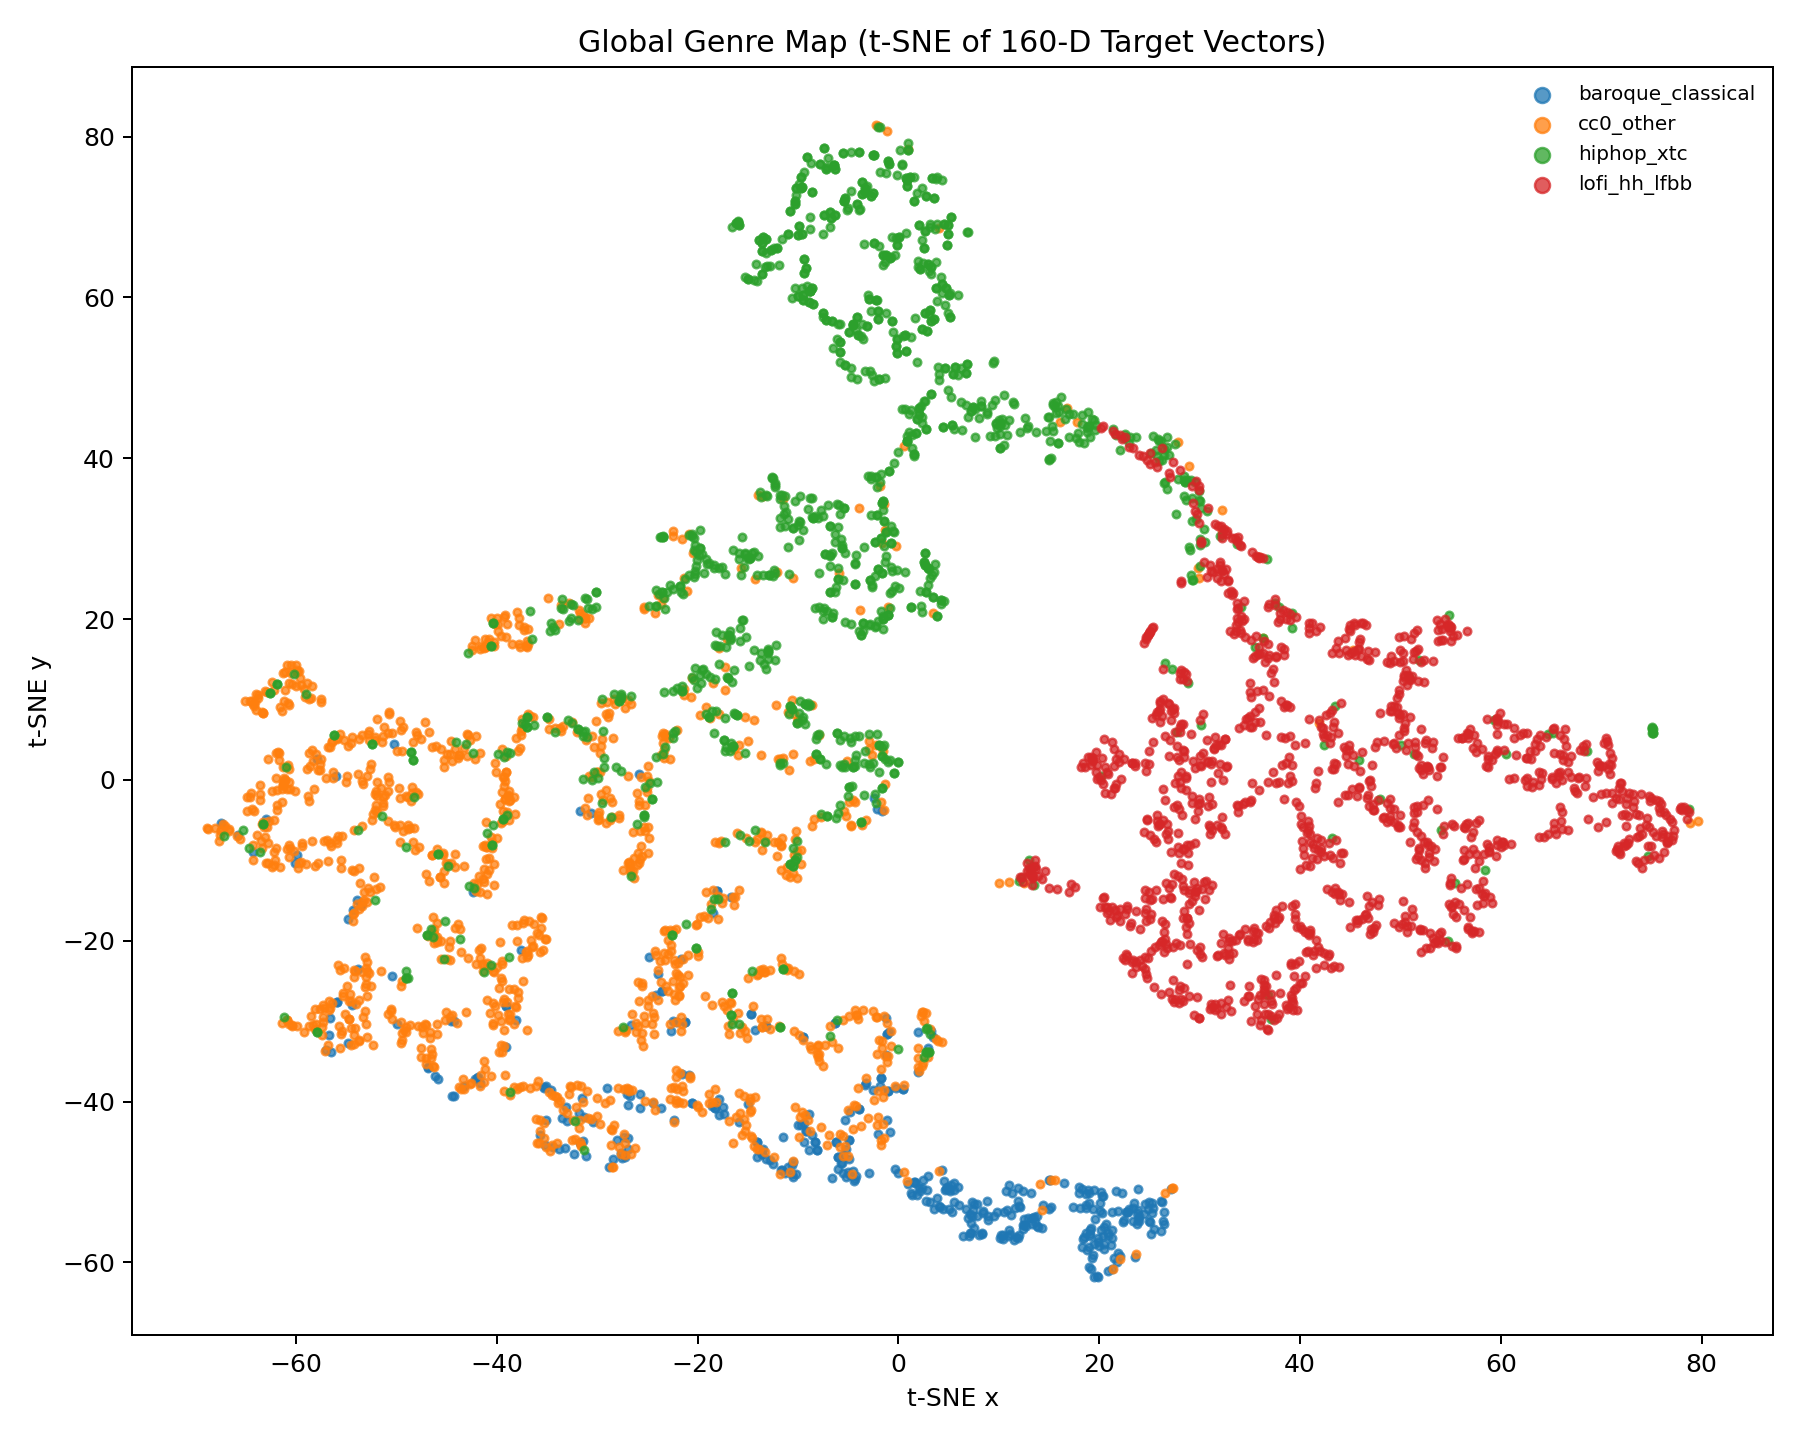
\includegraphics[width=\linewidth,height=0.72\textheight,keepaspectratio]{assets/lab2_tsne.png}
\end{columns}

\vspace{0.06cm}
\refstrip{The visualization comes from current repo calibration artifacts, not from an external paper figure.}
\end{frame}

\begin{frame}{Lab 2: Validation and Interpretation}
\begin{columns}[T,onlytextwidth]
  \column{0.5\textwidth}
  \cardbox{Mist}{
    \textbf{Current validation metrics}\\[-0.2em]
    \small
    linear probe accuracy: \textbf{0.8554}\\
    nearest centroid accuracy: \textbf{0.8514}\\
    silhouette (cosine): \textbf{0.4939}
  }
  \vspace{0.2cm}
  \cardbox{Paper}{
    \textbf{Completion gate}\\[-0.2em]
    \small
    The lab threshold was silhouette $\ge 0.45$. The current run clears it with margin.
  }

  \column{0.5\textwidth}
  \cardbox{Peach}{
    \textbf{Why this matters downstream}\\[-0.2em]
    \small
    A generator can only follow a style target if that target has stable geometry. Lab 2 is what makes the later conditioning story credible.
  }
  \vspace{0.2cm}
  \cardbox{Slate}{
    \textbf{Presentation lesson}\\[-0.2em]
    \small
    This is the best point in the talk to emphasize that representation quality is not separate from generation quality; it is upstream of it.
  }
\end{columns}
\end{frame}

\begin{frame}{Lab 3A: Codec-Latent Translator Architecture}
\begin{columns}[T,onlytextwidth]
  \column{0.58\textwidth}
  \begin{equation*}
  q_{\mathrm{src}} \in \mathbb{R}^{128 \times T},
  \qquad
  c = [z_c \,\|\, z_{s,\mathrm{tgt}} \,\|\, \eta],
  \qquad
  \eta \in \mathbb{R}^{32}
  \end{equation*}
  \begin{equation*}
  q_{\mathrm{hat}} =
  \begin{cases}
    q_{\mathrm{src}} + s\tanh(r) & \text{residual mode}\\
    r & \text{direct-output mode}
  \end{cases}
  \end{equation*}
  \cardbox{Paper}{
    \textbf{Implemented network}\\[-0.2em]
    \small
    Conv1D in-projection, hidden width 256, 10 residual FiLM blocks with dilations $[1,2,4,8,1,2,4,8,1,2]$, GroupNorm, SiLU, then a Conv1D back to 128 codec channels.
  }

  \column{0.42\textwidth}
  \cardbox{Mist}{
    \textbf{Why EnCodec matters}\\[-0.2em]
    \small
    The pretrained decoder acts as a realism prior. We edit a latent representation that already decodes to plausible audio instead of learning waveform physics from scratch.
  }
  \vspace{0.2cm}
  \cardbox{Peach}{
    \textbf{Important design decision}\\[-0.2em]
    \small
    Direct-output mode removes the identity shortcut that was capping style-shift magnitude in earlier residual runs.
  }
\end{columns}
\end{frame}

\begin{frame}{Lab 3A: Loss Stack and Best Run}
\begin{columns}[T,onlytextwidth]
  \column{0.6\textwidth}
  \begin{equation*}
  \begin{aligned}
  \mathcal{L}_{\mathrm{codec}} =
  &\lambda_{\mathrm{adv}}\mathcal{L}_{\mathrm{hinge\text{-}GAN}}
  + \lambda_{\mathrm{fm}}\mathcal{L}_{\mathrm{feat}}
  + \lambda_1 \|q_{\mathrm{hat}} - q^*\|_1 \\
  &+ \lambda_{\mathrm{mrstft}}\mathcal{L}_{\mathrm{MR\text{-}STFT}}
  + \lambda_c \mathcal{L}_{\mathrm{content}}
  + \lambda_s \mathcal{L}_{\mathrm{style}}
  + \lambda_p \mathcal{L}_{\mathrm{push}}
  \end{aligned}
  \end{equation*}
  \cardbox{Paper}{
    \textbf{Best saved run: \texttt{run1055}}\\[-0.2em]
    \small
    MPS: \textbf{0.9565}\\
    style confidence: \textbf{0.8940}\\
    style accuracy: \textbf{0.9492}
  }

  \column{0.4\textwidth}
  \cardbox{Mist}{
    \textbf{Why this branch is strong}\\[-0.2em]
    \small
    1. MERT probe embeddings improved target style conditioning.\\
    2. Direct-output translation enabled stronger edits.\\
    3. Explicit content loss kept the stronger edits from destroying melody.
  }
  \vspace{0.2cm}
  \cardbox{Slate}{
    \textbf{Current conclusion}\\[-0.2em]
    \small
    For short-form transfer, the codec branch is the strongest evidence path in the repo today.
  }
\end{columns}
\end{frame}

\begin{frame}{Lab 3B: Diffusion V2 Architecture}
\begin{columns}[T,onlytextwidth]
  \column{0.58\textwidth}
  \cardbox{Paper}{
    \textbf{Input tensor}\\[-0.2em]
    \small
    $[B,15,80,432] = 1$ noisy mel $+ 12$ chroma $+ 1$ onset $+ 1$ beat-grid channel
  }
  \vspace{0.18cm}
  \cardbox{Mist}{
    \textbf{Output tensor}\\[-0.2em]
    \small
    $[B,1,80,432]$ velocity/noise prediction for DDIM sampling
  }
  \vspace{0.18cm}
  \cardbox{Peach}{
    \textbf{UNet backbone}\\[-0.2em]
    \small
    channel progression $[64,128,256,256]$, two residual blocks per level, self-attention at low resolutions, EMA shadow model for sampling stability
  }

  \column{0.42\textwidth}
  \begin{equation*}
  \mathrm{cond}_{tc} = f_t(t) + f_c(z_c)
  \end{equation*}
  \begin{equation*}
  s = f_s(z_s)
  \end{equation*}
  \begin{equation*}
  h' = \mathrm{AdaIN}\bigl(\mathrm{FiLMResBlock}(h,\mathrm{cond}_{tc}), s\bigr)
  \end{equation*}
  \cardbox{Slate}{
    \textbf{Design rationale}\\[-0.2em]
    \small
    Time and content share a FiLM path for structure; style gets its own AdaIN path so timbre control does not overwhelm melody control.
  }
\end{columns}
\end{frame}

\begin{frame}{Diffusion Training Behavior and Checkpoint Selection}
\begin{columns}[T,onlytextwidth]
  \column{0.62\textwidth}
  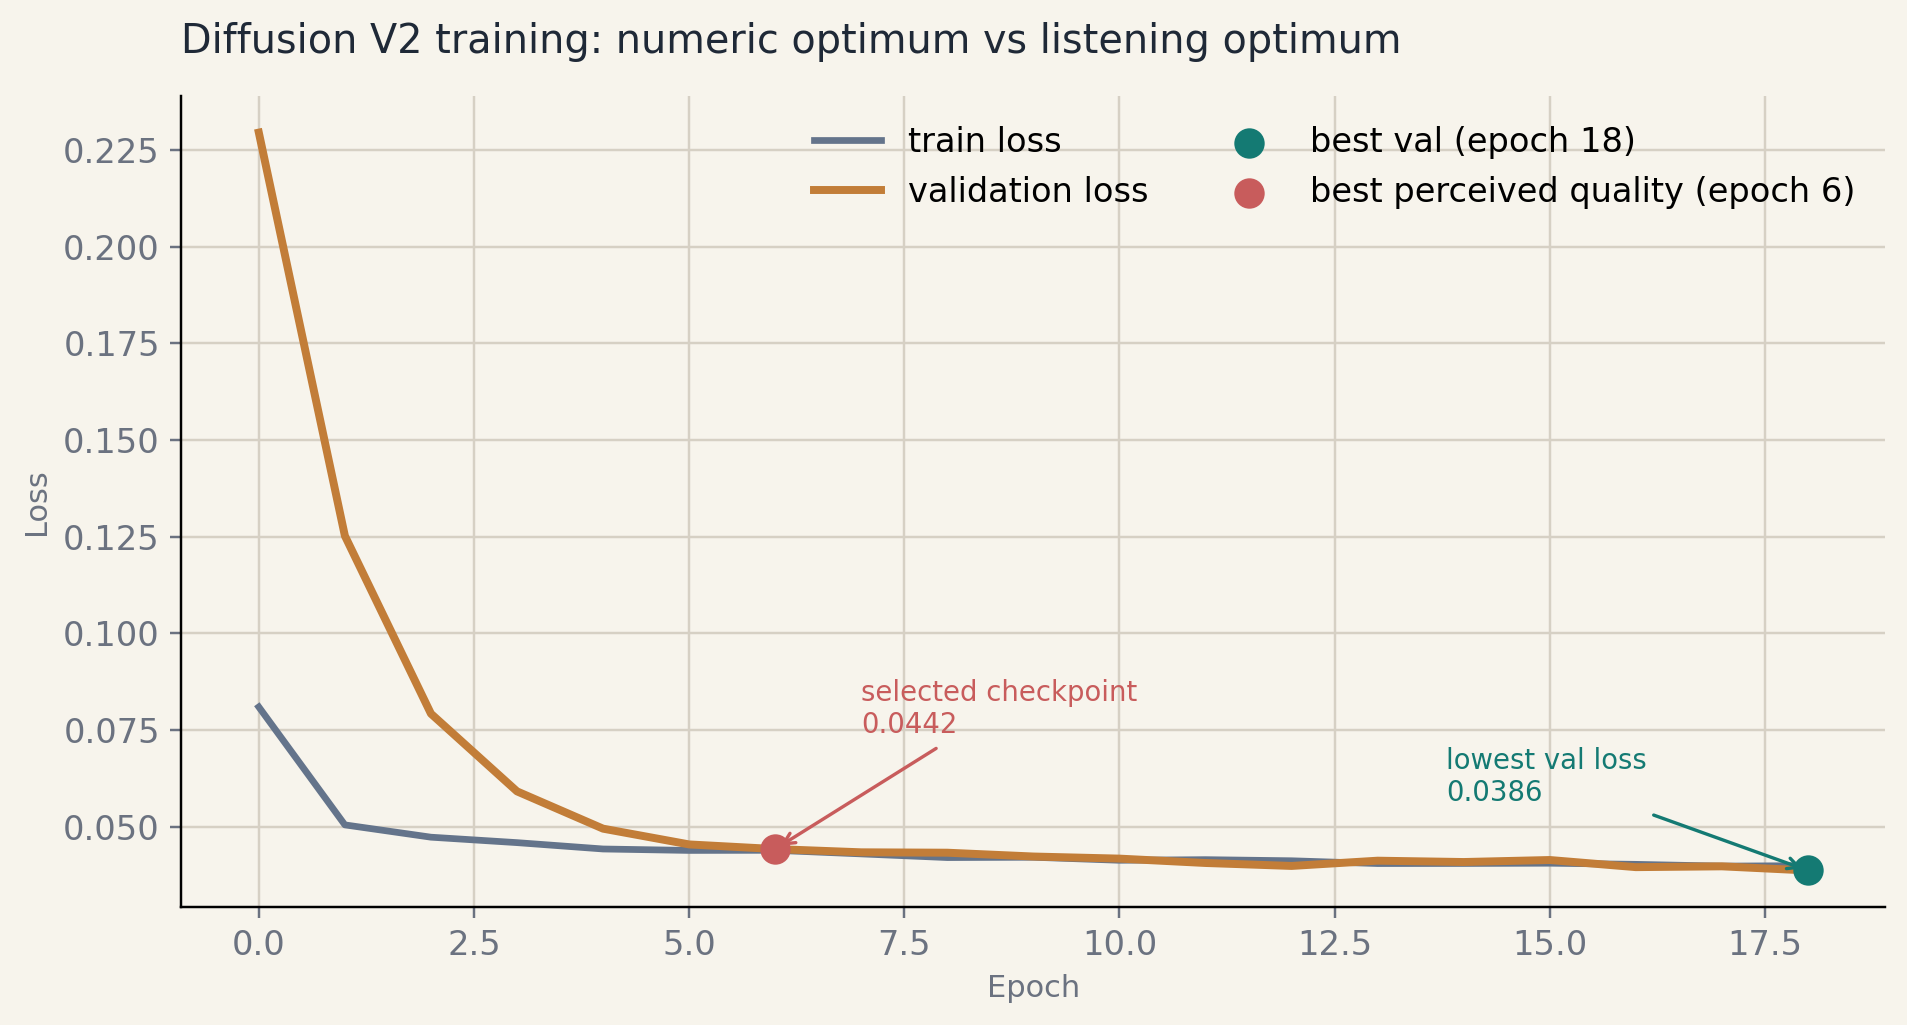
\includegraphics[width=\linewidth,height=0.58\textheight,keepaspectratio]{assets/diffusion_v2_curve.png}

  \column{0.38\textwidth}
  \cardbox{Mist}{
    \textbf{Observed behavior}\\[-0.2em]
    \small
    Validation loss kept improving through epoch 18, but the team selected epoch 6 as the best-sounding checkpoint for actual generation.
  }
  \vspace{0.2cm}
  \cardbox{Paper}{
    \textbf{Interpretation}\\[-0.2em]
    \small
    Later checkpoints appear numerically better but perceptually more averaged. This is why listening checkpoints belong in the workflow, not just in the final demo.
  }
\end{columns}
\end{frame}

\begin{frame}{Lab 4: Long-Form Coherence Method}
\begin{columns}[T,onlytextwidth]
  \column{0.58\textwidth}
  \begin{equation*}
  x_t^{(k)} = \alpha(t)x_0^{(k)} + \sigma(t)\epsilon
  \end{equation*}
  \begin{equation*}
  \mathrm{prefix}\!\left(x_t^{(k)}\right) \leftarrow \mathrm{tail}\!\left(x_t^{(k-1)}\right)
  \end{equation*}
  \cardbox{Paper}{
    \textbf{Implemented recipe}\\[-0.2em]
    \small
    1. Split the song into overlapping chunks.\\
    2. Forward-diffuse each chunk from the source mel instead of pure noise.\\
    3. At every DDIM step, lock the new chunk's overlap prefix to the previous chunk's overlap tail.\\
    4. Use re-anchoring and source blending to reduce drift.
  }

  \column{0.42\textwidth}
  \cardbox{Mist}{
    \textbf{Why not just crossfade?}\\[-0.2em]
    \small
    A crossfade can hide amplitude seams, but it does not solve semantic drift. Prefix locking tries to make adjacent chunks agree before vocoding.
  }
  \vspace{0.2cm}
  \cardbox{Slate}{
    \textbf{What this really is}\\[-0.2em]
    \small
    A sampling-policy contribution on top of the diffusion model, not just a post-processing trick.
  }
\end{columns}
\end{frame}

\begin{frame}{Lab 4: Diagnostics from the Full-Song Test}
\begin{columns}[T,onlytextwidth]
  \column{0.6\textwidth}
  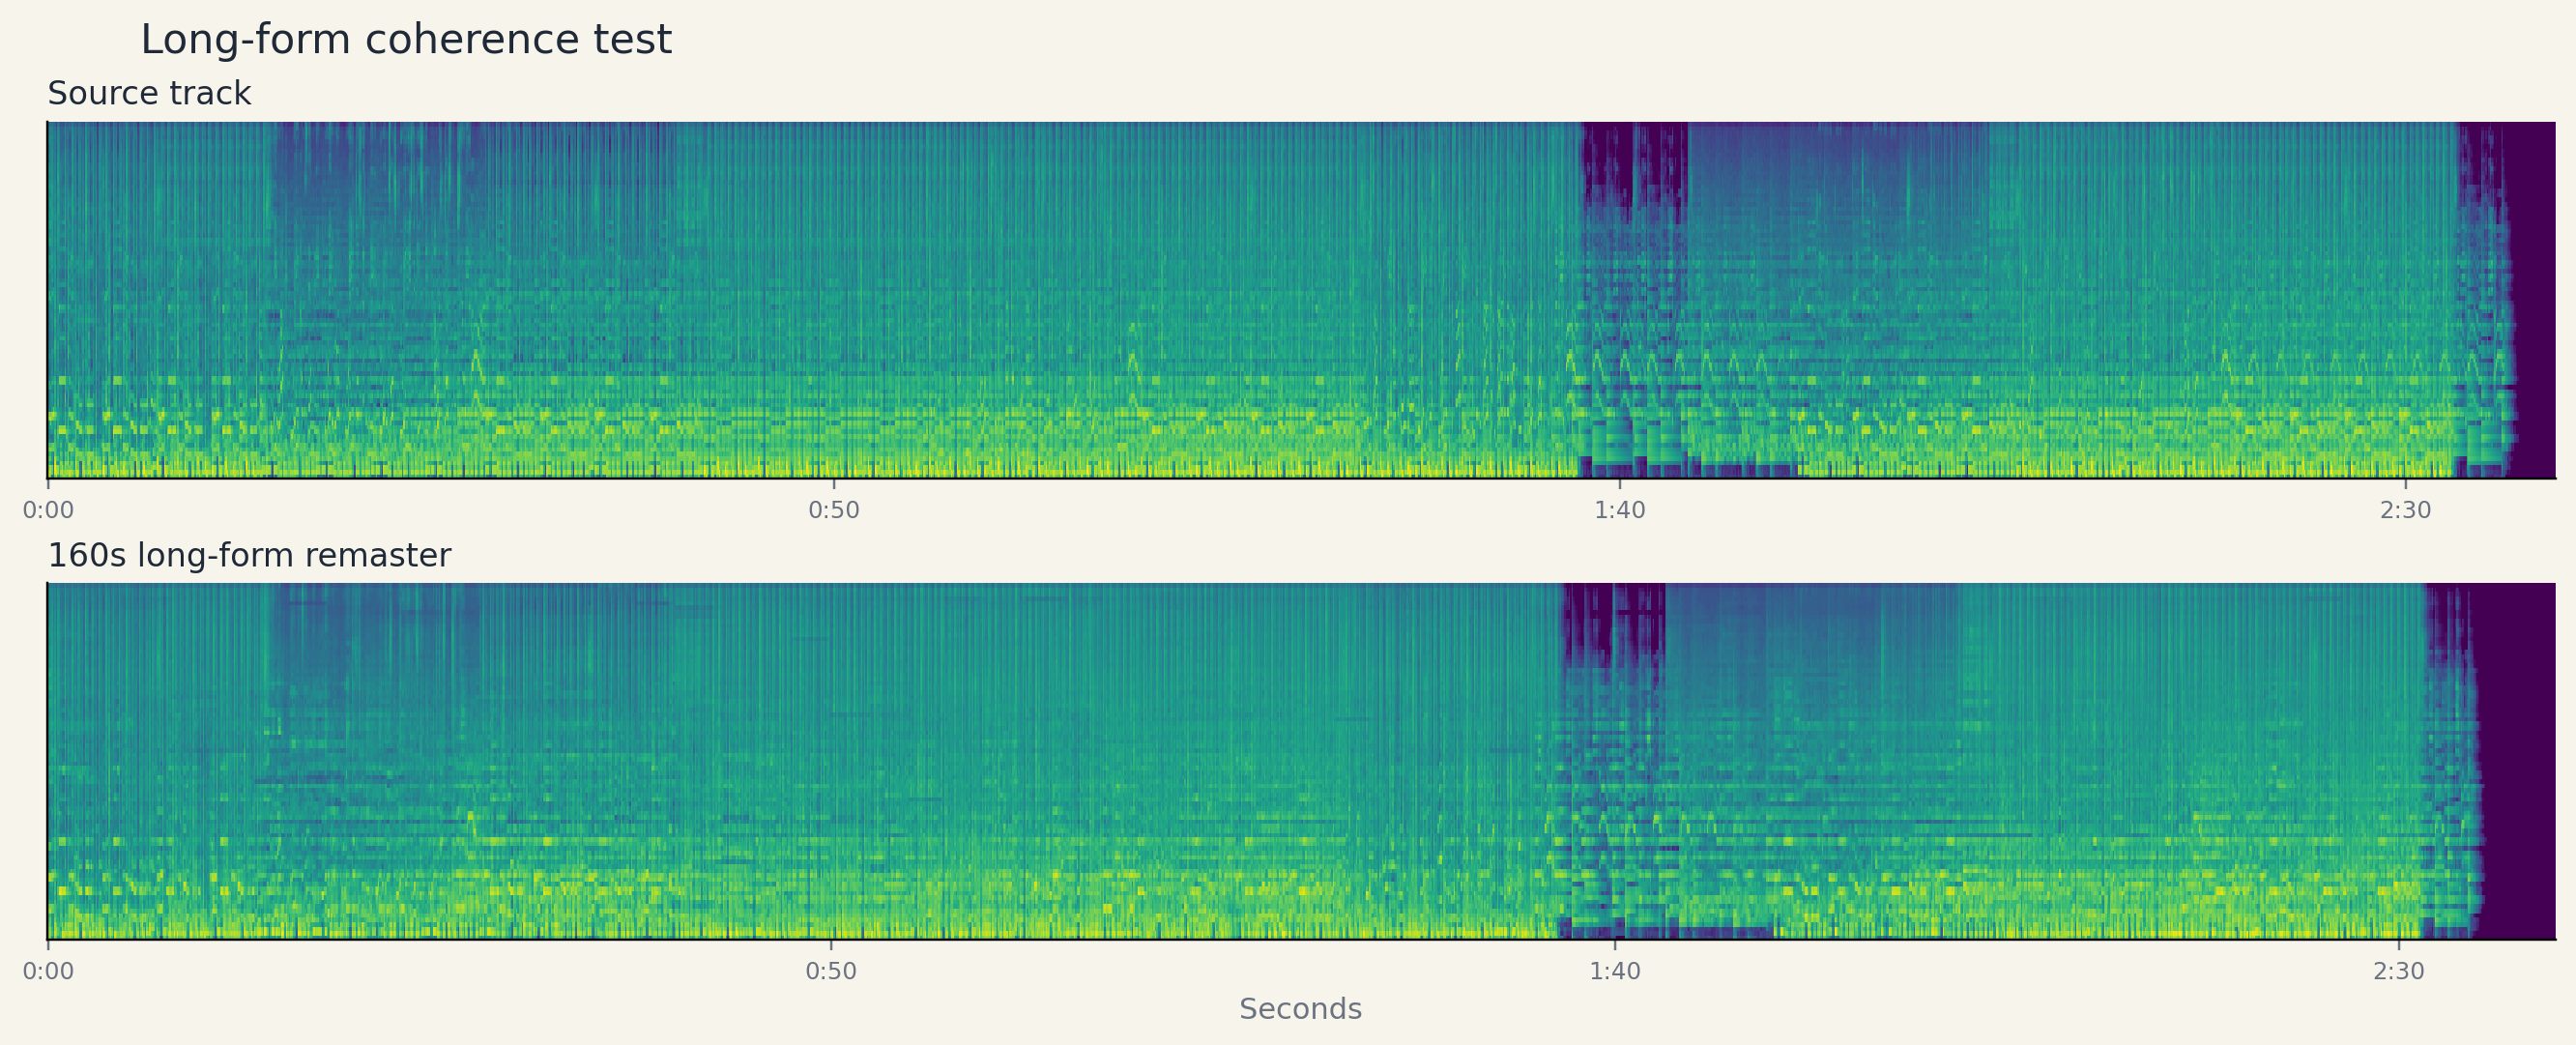
\includegraphics[width=\linewidth,height=0.56\textheight,keepaspectratio]{assets/longform_comparison.png}

  \column{0.4\textwidth}
  \cardbox{Paper}{
    \textbf{Current full-song test}\\[-0.2em]
    \small
    duration: \textbf{160 s}\\
    chunks: \textbf{64}\\
    boundary mel MSE mean: \textbf{0.00183}\\
    boundary discontinuity mean: \textbf{2.87 dB}
  }
  \vspace{0.2cm}
  \cardbox{Mist}{
    \textbf{Interpretation}\\[-0.2em]
    \small
    Overlap handling is helping. The remaining problem is mostly gradual warble and static accumulation rather than obvious seam cuts. Long-form quality depends on chunk policy, anchoring, vocoding, and stabilization together, not just on the base diffusion model.
  }
\end{columns}
\end{frame}

\begin{frame}{Quantitative Summary Across Labs}
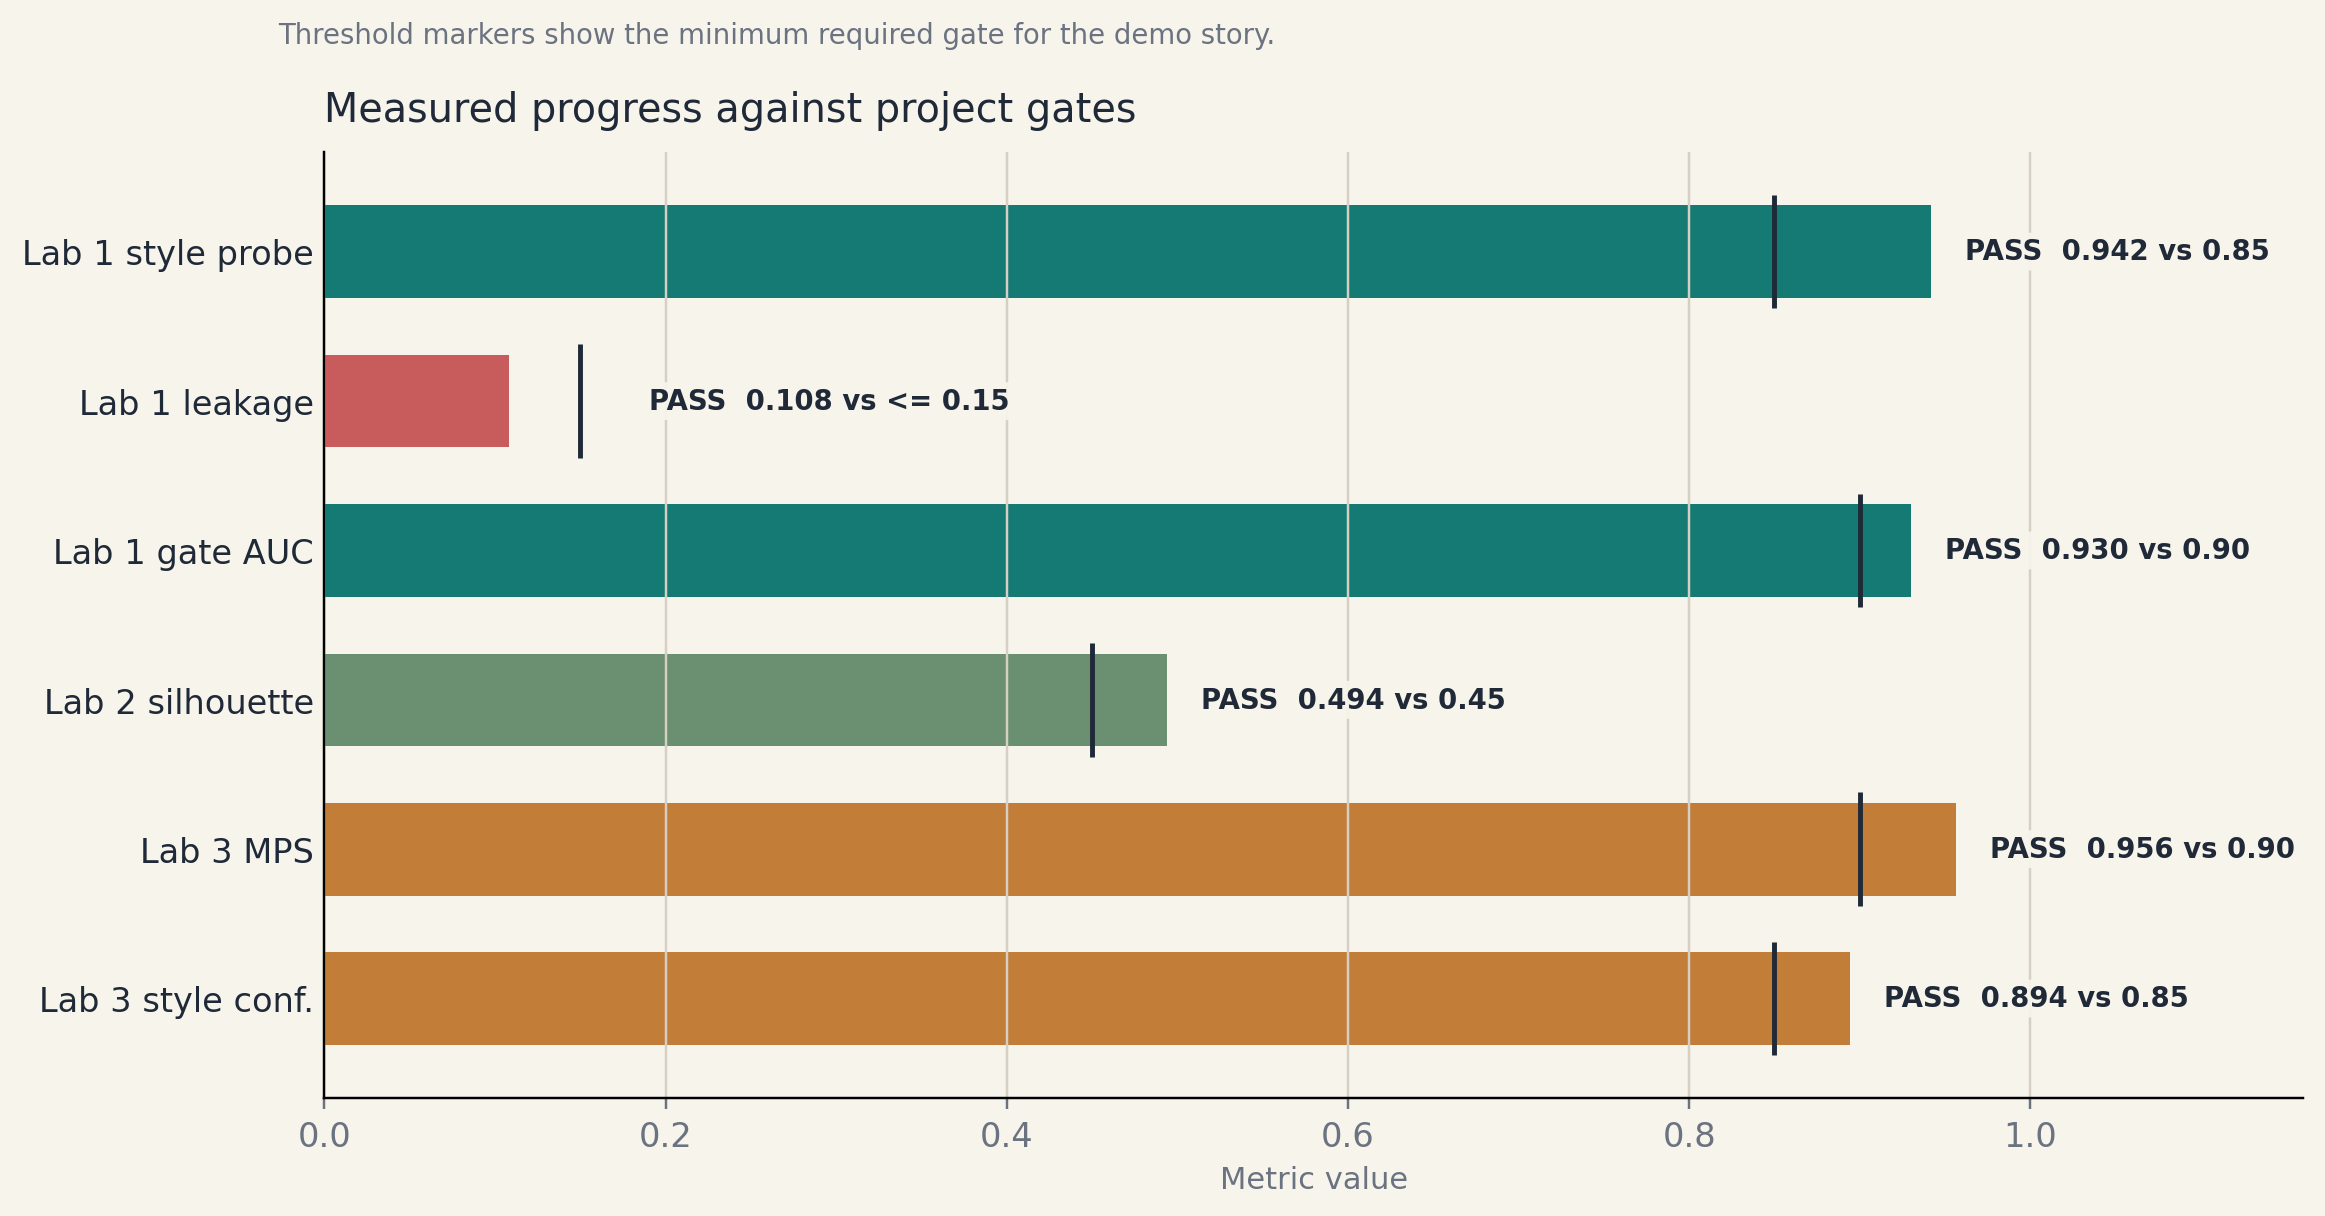
\includegraphics[width=\linewidth,height=0.5\textheight,keepaspectratio]{assets/metrics_dashboard.png}

\vspace{0.15cm}
\begin{columns}[T,onlytextwidth]
  \column{0.5\textwidth}
  \cardbox{Mist}{
    \textbf{Already strong}\\[-0.2em]
    \small
    Lab 1 and Lab 2 both clear their thresholds. The codec branch also clears the core short-form style and content gates.
  }
  \column{0.5\textwidth}
  \cardbox{Peach}{
    \textbf{Still open}\\[-0.2em]
    \small
    Better diffusion audio quality, stronger long-form texture stability, and a finished blind listening study in Lab 5.
  }
\end{columns}
\end{frame}

\begin{frame}{Audio Demo I: Short-Form Codec Examples}
\begin{columns}[T,onlytextwidth]
  \column{0.58\textwidth}
  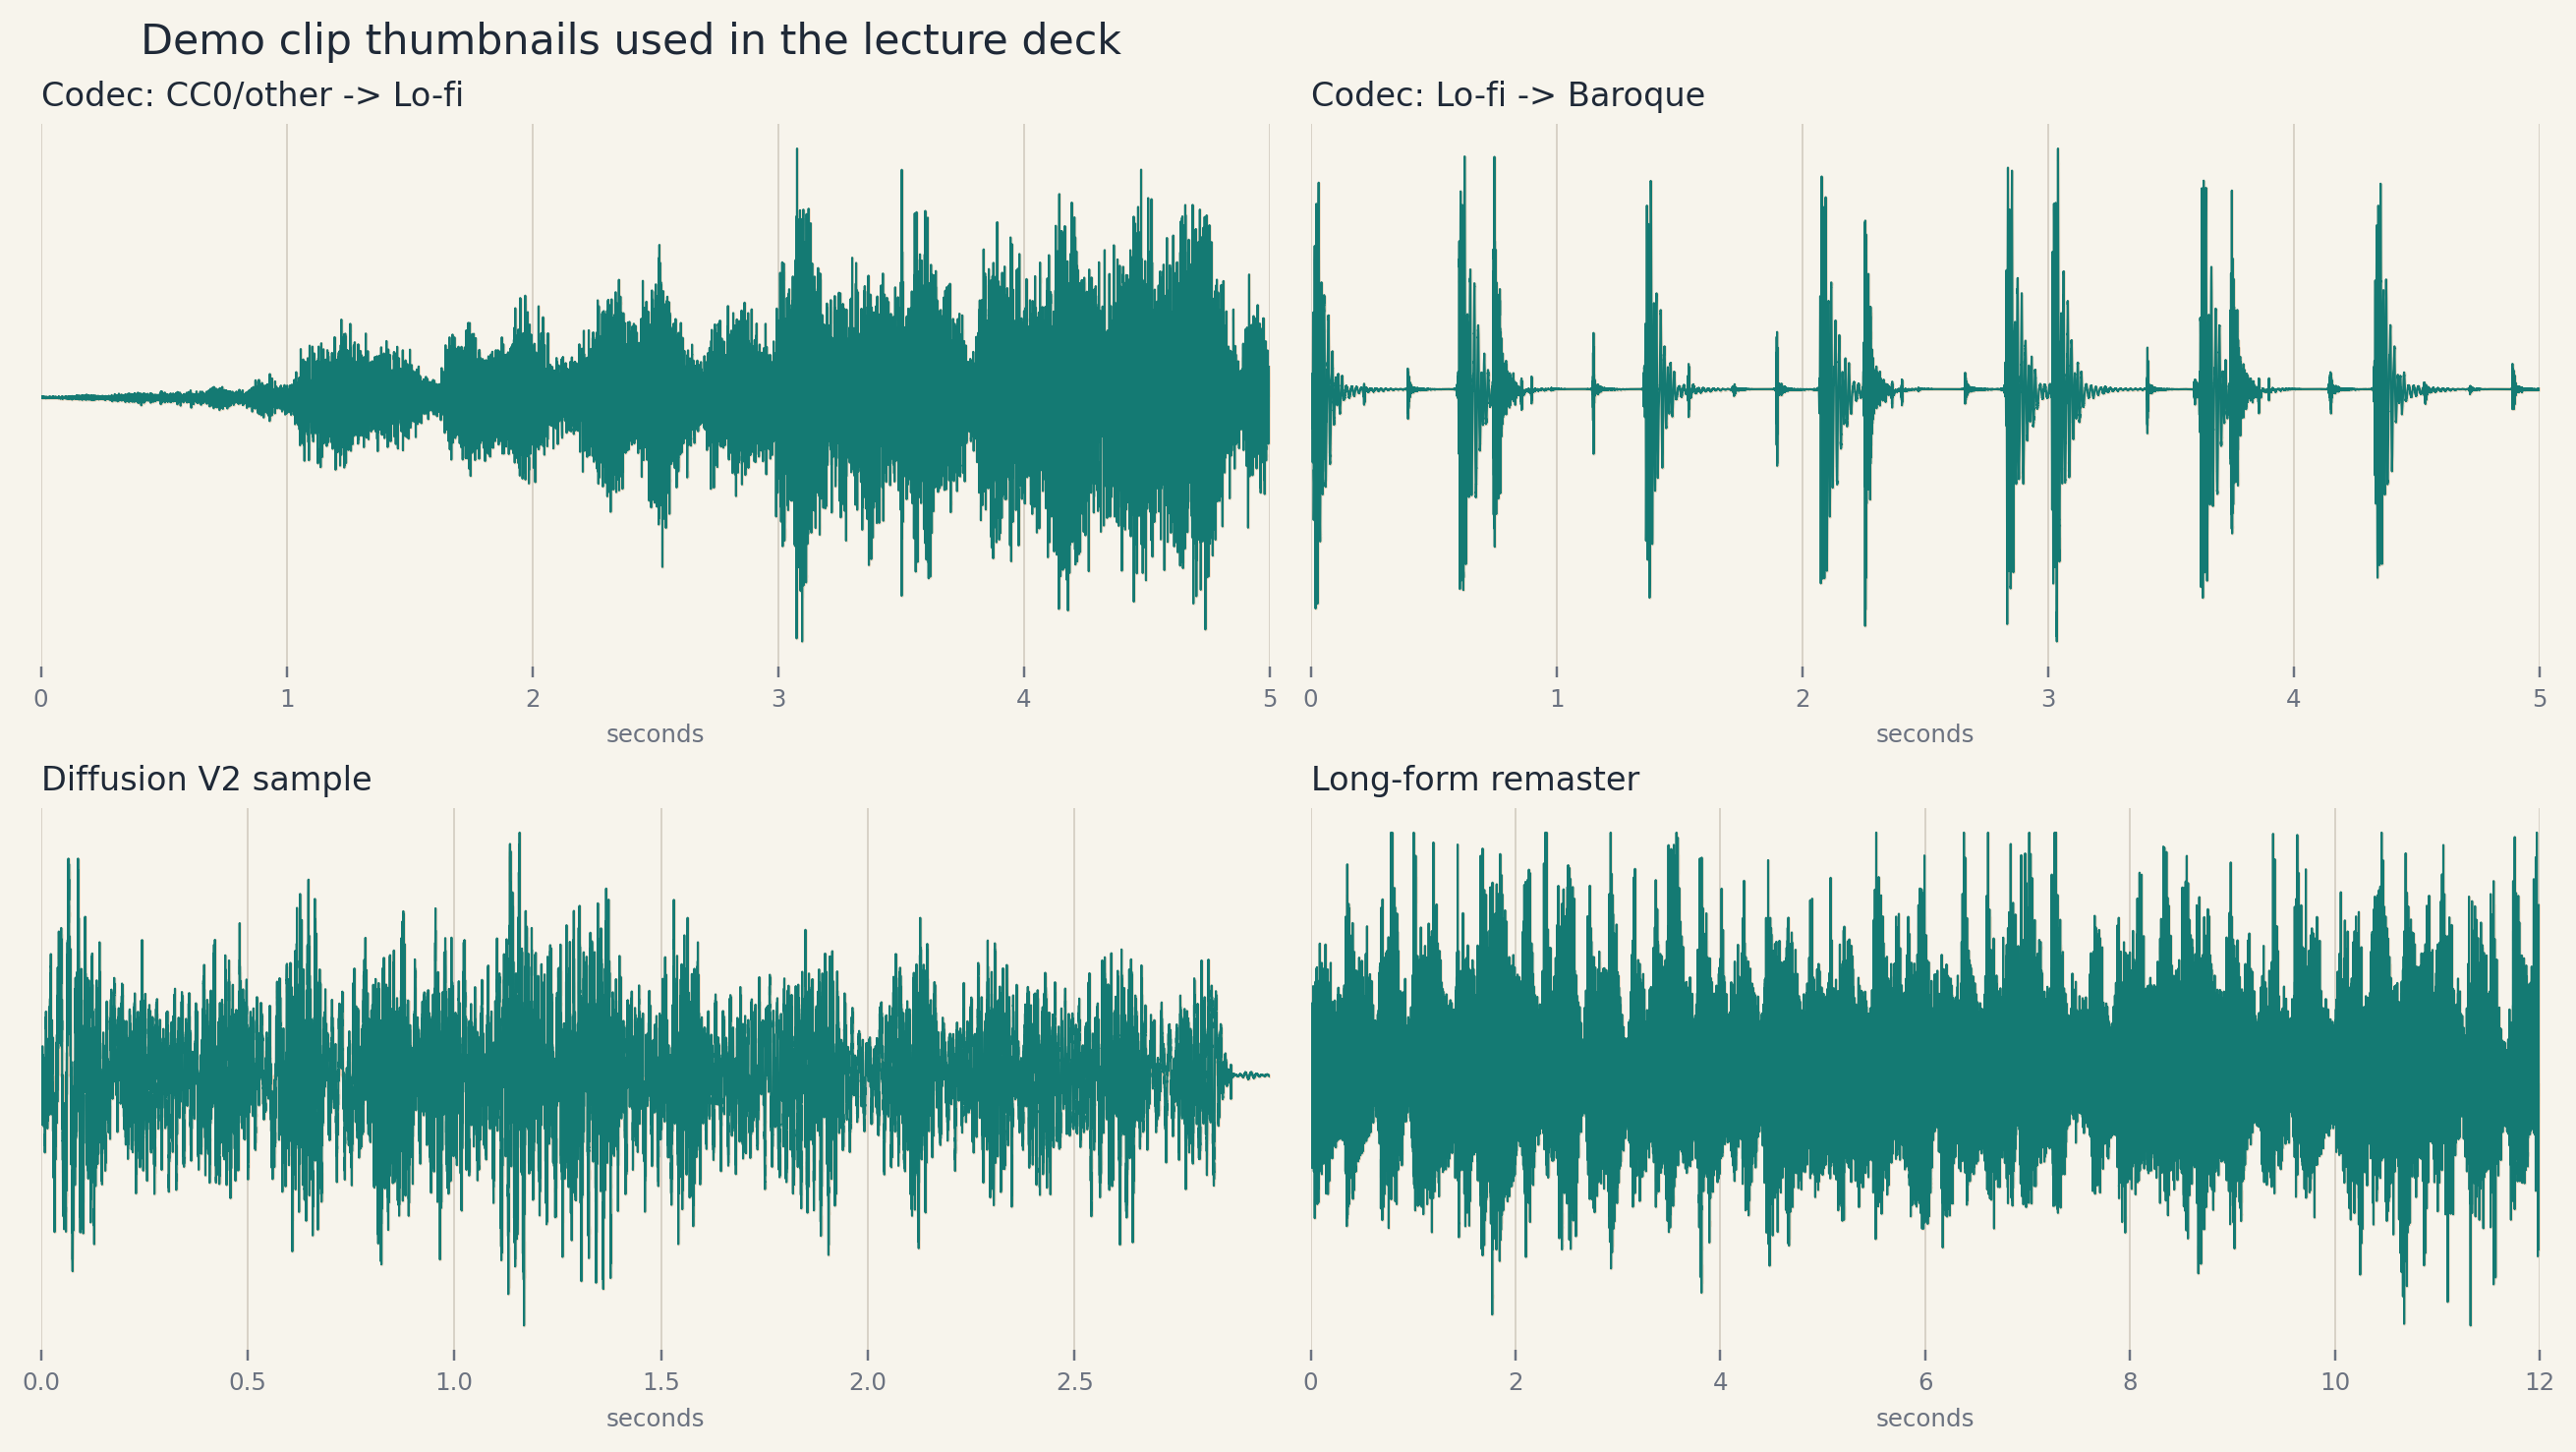
\includegraphics[width=\linewidth,height=0.58\textheight,keepaspectratio]{assets/demo_audio_grid.png}

  \column{0.42\textwidth}
  \cardbox{Paper}{
    \textbf{Clips from \texttt{run1055}}\\[-0.2em]
    \small
    CC0 other to lo-fi\\
    \AudioButton{media/codec_src1_tgt3.mp3}{clip 1}{5 s}\\[0.16cm]
    hip-hop to open-domain other\\
    \AudioButton{media/codec_src2_tgt1.mp3}{clip 2}{5 s}\\[0.16cm]
    lo-fi to baroque\\
    \AudioButton{media/codec_src3_tgt0.mp3}{clip 3}{5 s}
  }
  \vspace{0.2cm}
  \cardbox{Mist}{
    \textbf{What to listen for}\\[-0.2em]
    \small
    Does the melody survive? Is the target genre perceptible? Does the result sound like plausible audio rather than a synthetic artifact?
  }
\end{columns}
\end{frame}

\begin{frame}{Audio Demo II: Diffusion and Long-Form Excerpts}
\begin{columns}[T,onlytextwidth]
  \column{0.55\textwidth}
  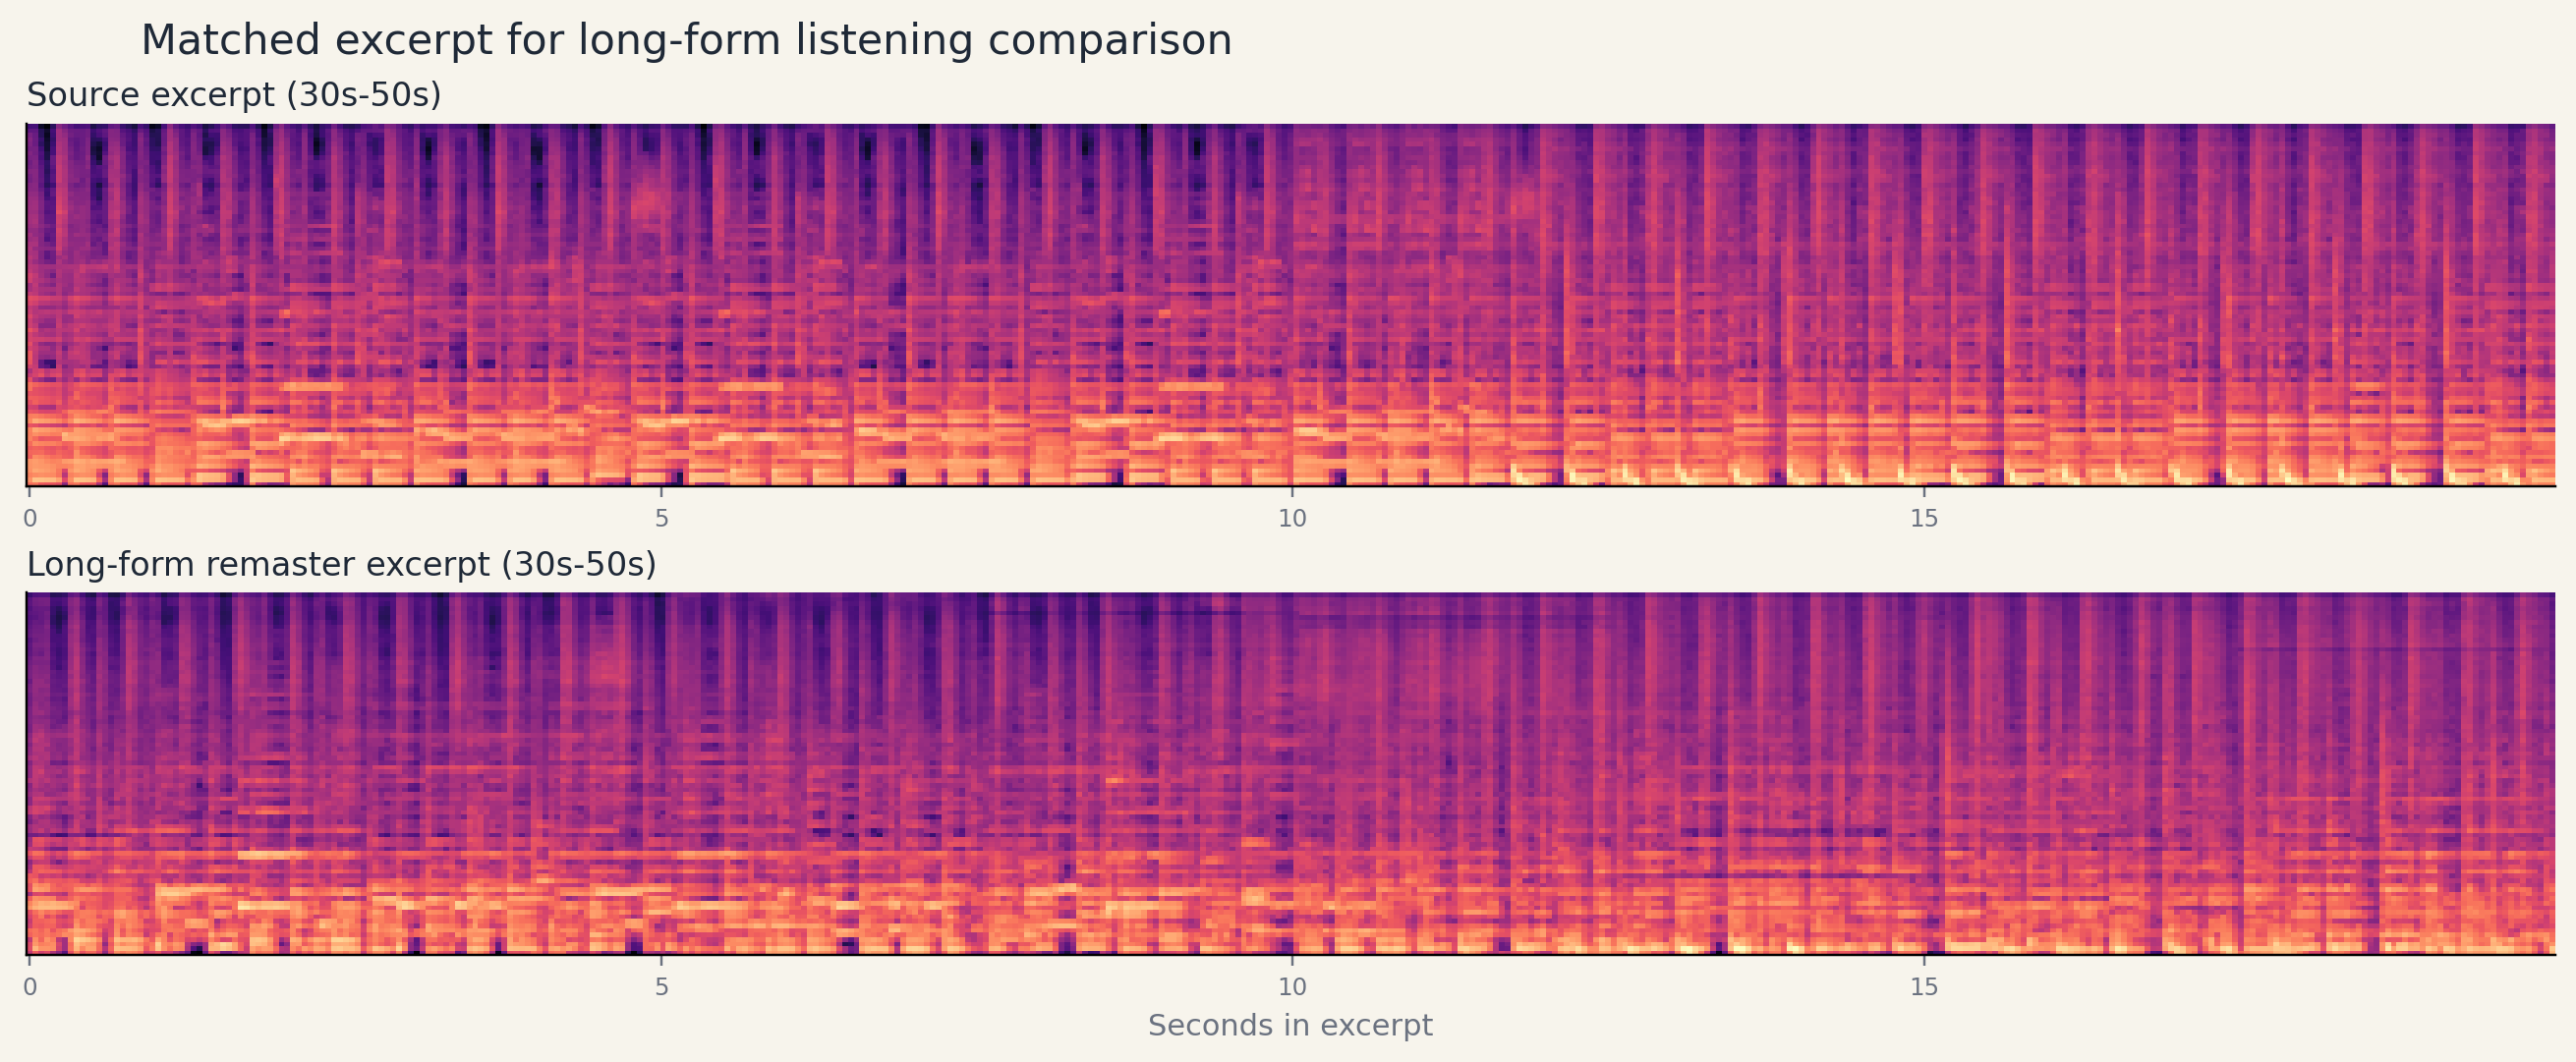
\includegraphics[width=\linewidth,height=0.56\textheight,keepaspectratio]{assets/longform_excerpt_comparison.png}

  \column{0.45\textwidth}
  \cardbox{Peach}{
    \textbf{Diffusion clip}\\[-0.2em]
    \small
    \AudioButton{media/diffusion_v2_epoch6_gen0.mp3}{Diffusion V2 sample}{3 s}
  }
  \vspace{0.2cm}
  \cardbox{Paper}{
    \textbf{Long-form A/B excerpt}\\[-0.2em]
    \small
    Source excerpt, 30 s--50 s\\
    \AudioButton{media/longform_source_excerpt.mp3}{source}{20 s}\\[0.16cm]
    Remastered excerpt, same segment\\
    \AudioButton{media/longform_remaster_excerpt.mp3}{remaster}{20 s}
  }
  \vspace{0.2cm}
  \cardbox{Mist}{
    \textbf{What to focus on}\\[-0.2em]
    \small
    Diffusion clip: edit freedom and texture.\\
    Long-form pair: continuity and artifact buildup.
  }
\end{columns}
\end{frame}

\begin{frame}{Creative Elements and Novelty}
\begin{columns}[T,onlytextwidth]
  \column{0.5\textwidth}
  \cardbox{Mist}{
    \textbf{Creative / novel components}\\[-0.2em]
    \small
    1. Structure-first framing of genre remastering instead of shallow timbre swapping.\\
    2. A staged pipeline with explicit deconstruction, calibration, reconstruction, and coherence stages.\\
    3. Direct-output codec translation plus MERT-based conditioning.\\
    4. Prefix-lock coherence constraints inside diffusion sampling.
  }
  \vspace{0.2cm}
  \cardbox{Paper}{
    \textbf{Why these count}\\[-0.2em]
    \small
    They are documented engineering responses to observed bottlenecks in the repo, not generic off-the-shelf invocations.
  }

  \column{0.5\textwidth}
  \cardbox{Peach}{
    \textbf{How to present this}\\[-0.2em]
    \small
    Emphasize that the novelty is not one isolated block. It is the combination of representation learning, stronger conditional translation, and long-form sampling controls.
  }
  \vspace{0.2cm}
  \cardbox{Slate}{
    \textbf{Creative-elements angle for CMPUT 414}\\[-0.2em]
    \small
    The project contributes new engineering structure and tuning decisions rather than merely re-running a known model with default settings.
  }
\end{columns}
\end{frame}

\begin{frame}{Limitations and Lab 5}
\begin{columns}[T,onlytextwidth]
  \column{0.5\textwidth}
  \cardbox{Peach}{
    \textbf{Current limitations}\\[-0.2em]
    \small
    1. Dataset-source leakage is still a genre-label risk.\\
    2. Diffusion quality currently lags codec transfer on short-form reliability.\\
    3. Long-form audio still accumulates warble and static under stronger edits.
  }
  \vspace{0.2cm}
  \cardbox{Slate}{
    \textbf{Lab 5 next step}\\[-0.2em]
    \small
    Run a blind listening study against simpler filter-style baselines and report both subjective genre authenticity and objective realism proxies.
  }

  \column{0.5\textwidth}
  \cardbox{Mist}{
    \textbf{What the final study should answer}\\[-0.2em]
    \small
    Can listeners identify the target genre? Can they still recognize the source melody? Do they prefer our remaster to a simpler baseline?
  }
  \vspace{0.2cm}
  \cardbox{Paper}{
    \textbf{Why this is the right ending}\\[-0.2em]
    \small
    At this point the key open question is no longer whether the architecture runs. It is whether people actually hear the intended effect.
  }
\end{columns}
\end{frame}

\begin{frame}{Conclusion}
\begin{columns}[T,onlytextwidth]
  \column{0.58\textwidth}
  \cardbox{Paper}{
    \textbf{Lecture takeaway}\\[-0.2em]
    \small
    Serious music style transfer is not one trick. It needs a representation story, a conditioning story, a synthesis story, and a coherence story.
  }
  \vspace{0.2cm}
  \cardbox{Mist}{
    \textbf{Case-study takeaway}\\[-0.2em]
    \small
    DGGR already clears its short-form technical gates and extends into measurable long-form coherence. The remaining gap is mainly perceptual refinement and formal human evaluation.
  }

  \column{0.42\textwidth}
  \cardbox{Peach}{
    \textbf{One-sentence summary}\\[-0.2em]
    \small
    We started from the general problem of meaningful genre transfer and built a repo-backed system that implements one defensible answer end-to-end.
  }
  \vspace{0.2cm}
  \cardbox{Slate}{
    \textbf{Discussion prompts}\\[-0.2em]
    \small
    Codec editing, diffusion, or hybrid?\\
    How should music evaluation balance taste with repeatability?
  }
\end{columns}
\end{frame}

\appendix

\begin{frame}[noframenumbering]{Backup: Exact Codec Branch Dimensions}
\small
\begin{tabularx}{\linewidth}{>{\raggedright\arraybackslash}p{3.6cm}X}
\toprule
\textbf{Component} & \textbf{Implementation detail} \\
\midrule
Input latents & EnCodec quantized embeddings, approximately $[B,128,T]$ \\
Condition vector & $z_c \in \mathbb{R}^{128}$, target style embedding $z_s \in \mathbb{R}^{128}$, noise $\eta \in \mathbb{R}^{32}$ \\
Hidden width & 256 channels \\
Residual stack & 10 FiLM-conditioned residual Conv1D blocks \\
Dilations & $[1,2,4,8,1,2,4,8,1,2]$ \\
Normalization & GroupNorm with 8 groups \\
Output mode & residual or direct-output translation; best run uses direct-output \\
Adversarial path & multi-scale waveform discriminator with hinge loss and feature matching \\
\bottomrule
\end{tabularx}
\end{frame}

\begin{frame}[noframenumbering]{Backup: Exact Diffusion Branch Dimensions}
\small
\begin{tabularx}{\linewidth}{>{\raggedright\arraybackslash}p{3.7cm}X}
\toprule
\textbf{Component} & \textbf{Implementation detail} \\
\midrule
Input tensor & $[B,15,80,432] = 1$ noisy mel $+ 12$ chroma $+ 1$ onset $+ 1$ beat channel \\
Output tensor & $[B,1,80,432]$ velocity/noise prediction \\
UNet channels & $[64,128,256,256]$ \\
Residual blocks & 2 per resolution level \\
Attention & lower resolutions in the current code path \\
Condition split & time and content via FiLM, style via dedicated AdaIN \\
Schedule & cosine beta schedule, DDIM sampling, EMA shadow model \\
Waveform path & BigVGAN-compatible mel extraction and waveform reconstruction \\
\bottomrule
\end{tabularx}
\end{frame}

\begin{frame}[noframenumbering]{Backup: Repo Evidence Used for This Lecture}
\small
\textbf{Core repo-backed evidence}\\
\footnotesize
Lab 1 explanations and audits in \texttt{docs/explanation/lab1\_deconstruction\_encoder.md} and \texttt{saves/lab1\_run\_combo\_af\_gate\_exit\_v2/}.\\
Lab 2 calibration artifacts in \texttt{saves/lab2\_calibration/lab2\_20260211\_015118\_lda\_cleanup\_v2/}.\\
Codec branch code in \texttt{dggr/lab3\_codec\_models.py}; best metrics in \texttt{saves2/lab3\_codec\_transfer/run1055/}.\\
Diffusion branch code in \texttt{dggr/lab3\_diffusion\_model.py}; training history in \texttt{saves2/lab3\_diffusion/run\_d002/}.\\
Long-form coherence code in \texttt{lab 3/run\_lab4\_longform\_coherence.py}; diagnostics in \texttt{saves2/lab4\_longform\_coherence/fullsong\_test/}.

\vspace{0.35cm}
\textbf{Visual and media assets}\\
\footnotesize
Charts and spectrograms were generated locally from repo artifacts using \texttt{presentation/generate\_figures.py}. Audio demo clips were converted from existing repo outputs into \texttt{presentation/media/}. OpenMoji icons are used through the local LaTeX package.
\end{frame}

\begin{frame}[noframenumbering]{Backup: Lecture References}
\footnotesize
Dai et al. (2018), Aucouturier and Pachet (2003), Ghosal and Kolekar (2018), Hung et al. (2019), Yang et al. (2019), Roberts et al. (2018), Donahue et al. (2019), Gulrajani et al. (2017), Engel et al. (2019), Lee et al. (2023), Perez et al. (2018), Ho et al. (2020), Ho and Salimans (2021), Borsos et al. (2023), Meng et al. (2022).
\end{frame}

\end{document}
